%%%%%%%%%%%%%%%%%%%%%%%%%%%%%%%%%%%%%%%%%%%%%%%%%%%%%%%%%%%
% AUTOR: DIOGO CEZAR TEIXEIRA BATISTA                     %   
% DATA: OUTUBRO-2010                                      % 
% LIVRO: INTRODU��O A TEORIA DOS GRAFOS E SEUS ALGORITMOS %
%%%%%%%%%%%%%%%%%%%%%%%%%%%%%%%%%%%%%%%%%%%%%%%%%%%%%%%%%%%

\documentclass[9pt,openany,twoside,a4paper]{extbook}
\usepackage[brazil]{babel}
\usepackage[latin1]{inputenc}
\usepackage[pdftex]{graphicx}
\usepackage[boxruled,noline,linesnumbered,portuguese,onelanguage,algoruled]{algorithm2e}
\usepackage{wrapfig}
\usepackage{fancyhdr}
\usepackage{color}
\usepackage{ifthen}
\usepackage{amsmath}
\usepackage{amsfonts}
\usepackage{amssymb}
\usepackage{indentfirst}
\usepackage{listings}
\usepackage[lmargin=2.5cm,rmargin=2.5cm,tmargin=2.5cm,bmargin=3.5cm]{geometry}
\usepackage{times}
\usepackage[T1]{fontenc}
\usepackage{avant}
\renewcommand*\familydefault{\sfdefault}

%%%%%%%%%%%%%%%%%%%%%%%%%%%%%%%%%%%%%%%%%%%%%%%%%%%%%%%%%%%
% C O N F I G U R A � � E S  D O S   A L G O R I T M O S  %
%%%%%%%%%%%%%%%%%%%%%%%%%%%%%%%%%%%%%%%%%%%%%%%%%%%%%%%%%%%

\IncMargin{0.2cm}
\SetNlSkip{0.1cm}

%%%%%%%%%%%%%%%%%%%%%%%%%%%%%%%%%%%%%%%%%%%%%
% E S P A � A M E N T O   A U M E N T A D O %
%%%%%%%%%%%%%%%%%%%%%%%%%%%%%%%%%%%%%%%%%%%%%

\renewcommand{\baselinestretch}{1.4}

%%%%%%%%%%%%%%%%%%%%%%%%%%%%%%%%%%%%%%%%%%%%%%%%%%%
% C O M A N D O S   D E   S U B S T I T U I � � O %
%%%%%%%%%%%%%%%%%%%%%%%%%%%%%%%%%%%%%%%%%%%%%%%%%%%

\newcommand{\titulo}        [1]{\def\imprimetitulo{#1}}
\newcommand{\subtitulo}     [1]{\def\imprimesubtitulo{#1}}
\newcommand{\autor}         [1]{\def\imprimeautor{#1}}

%%%%%%%%%%%%%%%%%%%%%%%%%%%%%%%%%%%%%%%%%%%%%%%%%%
%  S U B S T I T U I N D O   C O N S T A N T E S %
%%%%%%%%%%%%%%%%%%%%%%%%%%%%%%%%%%%%%%%%%%%%%%%%%%

\titulo{INTRODU��O A TEORIA DOS GRAFOS E SEUS ALGORITMOS}
\subtitulo{Uma vis�o introdut�ria da teoria dos grafos}
\autor{Diogo Cezar Teixera Batista \\ \vspace{0.5cm}  Robson Gomes de Melo \\ \vspace{0.7cm} Andr� Luiz Pires Guedes}

%%%%%%%%%%%%%%%%%%%%%%%%%%%%%%%%%%%%%%%%%%%%%%%%%%%%%%%%%%
% C O N F I G U R A N D O   O   F A N C Y   H E A D E R  %
%%%%%%%%%%%%%%%%%%%%%%%%%%%%%%%%%%%%%%%%%%%%%%%%%%%%%%%%%%

\pagestyle{fancy}                       
\fancyfoot{}                            
\renewcommand{\chaptermark}[1]{         
  \markboth{\chaptername\ \thechapter.\ #1}{}}
\renewcommand{\sectionmark}[1]{         
  \markright{\thesection.\ #1}}         
\fancyhead[LE,RO]{\bfseries\thepage}    

\fancyhead[RE]{\bfseries\leftmark}      
\fancyhead[LO]{\bfseries\rightmark}     
\renewcommand{\headrulewidth}{0.3pt}    

\makeatletter 
\def\cleardoublepage{\clearpage\if@twoside \ifodd\c@page\else% 
    \hbox{} 
    \thispagestyle{empty}
    \newpage 
    \if@twocolumn\hbox{}\newpage\fi\fi\fi} 
\makeatother

%%%%%%%%%%%%%%%%%%%%%%%%%%%%%%%%%%%%%%%%%
% R O D A P �  C O M   C O N T E � D O  %
%%%%%%%%%%%%%%%%%%%%%%%%%%%%%%%%%%%%%%%%%

\newcommand{\setfooter}{
    \pagestyle{fancy}
    \lfoot{}
    \cfoot{\thepage}
    \rfoot{}
}

\begin{document}

%%%%%%%%%%%
% C A P A %
%%%%%%%%%%%

    \begin{flushright}
    \end{flushright}

    \thispagestyle{empty}

    \vspace{3cm}

    \begin{center}
    {\Huge \textbf{\imprimetitulo}}

    \vspace{5cm}

    {\huge \textbf{\imprimesubtitulo}}

    \vspace{5cm}

    {\Large \imprimeautor}

    \vspace{2cm}

    \end{center}

    \newpage

%%%%%%%%%%%%%%%%%%%
% S U M � R I O S %
%%%%%%%%%%%%%%%%%%%

    \thispagestyle{empty}

    \tableofcontents

    \newpage

    \thispagestyle{empty}

    \listoffigures

    \newpage

    \setfooter

%%%%%%%%%%%%%%%%%%%%%%%%%%%%%%%%%%%%%%%%%%
% D O C U M E N T O   P R I N C I P A L  %
%%%%%%%%%%%%%%%%%%%%%%%%%%%%%%%%%%%%%%%%%%

    %%%%%%%%%%%%%%%%%%%%%%%
% C A P � T U L O   1 %
%%%%%%%%%%%%%%%%%%%%%%%

\chapter{Grafos - Defini��es Iniciais}

Para qualquer conjunto $V$, denotamos $\displaystyle\binom{V}{2}$ o conjunto de todos pares n�o-ordenados de elementos de $V$. Se $V$ tem $n$ elementos ent�o $\displaystyle\binom{V}{2}$ tem $\displaystyle\frac{n(n-1)}{2}$ elementos. Os elementos de $\displaystyle\binom{V}{2}$ ter� a forma $\{v,w\}$, sendo $v$ e $w$ dois elementos distintos de $V$.

Um grafo � um par ordenado de conjuntos finitos $(V,E)$ tal que $E \subseteq \binom{V}{2}$. Isso significa que cada elemento $E$ � um subconjunto de elementos de $V$ ou um bin�mio de $V$. Cada elemento de $V$ � chamado de \emph{v�rtice} do grafo e cada elemento de $E$ � chamado de \emph{aresta} do grafo, dessa forma cada aresta $e \in E$ � um subconjunto de $V$ formado por exatamente dois v�rtices, ou seja, $e \subseteq V$ e $|e| = 2$.

Todo grafo pode ser representado geometricamente por um diagrama. No plano, desenhamos um ponto para cada v�rtice e um segmento de curva ligando cada par de v�rtices que determinam uma aresta (Figura \ref{fig:g_1}). Claramente, essa representa��o geom�trica de um grafo n�o � �nica.

\paragraph*{Exemplo 1:} Os conjuntos:

\begin{eqnarray*}
    V &=& \{1,2,3,4,5,6,7,8\} \\
    E &=& \{\{1,2\},\{1,5\},\{2,5\},\{3,4\},\{6,7\}\}
\end{eqnarray*}

definem um grafo e um diagrama desse grafo � apresentado na Figura \ref{fig:g_1}.

\begin{figure}[!htb]
    \centering
    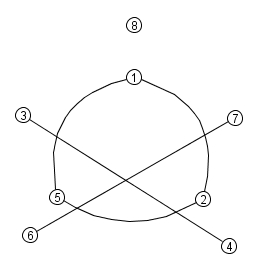
\includegraphics[width=4.5cm]{grafos_yed/g_1.jpg}
    \caption{Representa��o geom�trica (ou diagrama) do grafo.}
    \label{fig:g_1}
\end{figure}

Se $G$ denota o grafo que � definido pelo par $(V,E)$ ent�o escrevemos $G = (V,E)$.

No que segue $u$ e $v$ denotam v�rtices e $e$ e $f$ denotam arestas de um grafo:

\begin{itemize}
    \item se $v \in e$ ent�o dizemos que a aresta $e$ \emph{incide} em $v$;
    \item se ${u, v}$ � uma aresta, ent�o dizemos que $u$ e $v$ s�o v�rtices \emph{adjacentes};
    \item se $|e \cap f| = 1$, ent�o dizemos que $e$ e $f$ s�o arestas \emph{adjacentes}, em outras palavras, se existe um v�rtice $v$ que � comum (faz a intersec��o)  �s arestas $e$ e $f$ ent�o essas s�o arestas adjacentes.
    \item quando $e = {v,u}$, dizemos que $u$ e $v$ s�o os extremos da aresta $e$.
\end{itemize}

Quando nos referimos a um grafo conhecido $G$ sem especificarmos o conjunto dos v�rtices e o conjunto das arestas que definem $G$ esses passam a ser referidos como $V(G)$ e $E(G)$, respectivamente. Assim, se $G = (X,Y)$ ent�o $V(G) = X$ e $E(G) = Y$.

Para um grafo $G$ qualquer, chamamos $|V (G)|$ de ordem de $G$ e chamamos $|V (G)| + |E(G)|$ de tamanho de $G$.

Um expoente em $G$, quando $G$ � um grafo, denota a ordem de $G$, assim quando queremos ressaltar que $G$ � um grafo de ordem $n$, para algum $n \in \mathbb{N}$, escrevemos $G^n$.

Chamamos $G^0 = (\varnothing,\varnothing)$ de grafo vazio e todo grafo de ordem 1 de grafo trivial.

\section{Grafo Completo}

Um grafo � chamado de completo sobre $V$ se todo par de v�rtices de $V$ � uma aresta do grafo, ou formalmente $E = \binom{V}{2}$ para cada par de v�rtices $V(G) = \{x,y\}$ existe uma aresta que os liga. Um grafo completo � denotado por $K^n$.

Outra defini��o para \textbf{grafo completo} � um grafo que tem todas as arestas poss�veis em $E(G)$. $ K_n = (V, \binom{V}{2})$ onde $V = \{1,2,3,4,\ldots,n\}$.

S�o exemplos de grafos completos:


\begin{itemize}
  \item[$K_1$] $ = (V_{k1}, E_{k1}) \therefore V_{k1} = \{1\} \mbox{ e } E_{k1} = \{\{\varnothing, \varnothing\}\}$
  \item[$K_2$] $ = (V_{k2}, E_{k2}) \therefore V_{k2} = \{1,2\} \mbox{ e } E_{k2} = \{1,2\}$
  \item[$K_3$] $ = (V_{k3}, E_{k3}) \therefore V_{k3} = \{1,2,3\} \mbox{ e } E_{k3} = \{\{1,2\}, \{2,1\}, \{1,3\}\}$
\end{itemize}

As representa��es geom�tricas dos grafos est�o dispostas na Figura \ref{fig:g_5} na qual, $K_1$ � representado por $a$, $K_2$ � representado por $b$ e $K_3$ � representado por $c$.

\begin{figure}[!htb]
    \centering
    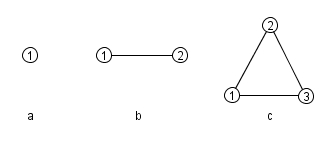
\includegraphics[width=6cm]{grafos_yed/g_5.jpg}
    \caption{Representa��o geom�trica (ou diagrama) dos grafos completos $K_1$, $K_2$ e $K_3$}
    \label{fig:g_5}
\end{figure}

As defini��es de $K$ para um $n$ completo representam um grafo com $n$ v�rtices completo, ent�o essa defini��o pode ser aplicada a todos os sucessivos grafos at� $K_n$.


\section{Complemento de um Grafo}

  O complemento de um grafo $G$, denotado por $\overline{G}$, � o grafo que tem o mesmo conjunto de \emph{v�rtices} de $G$ e dois v�rtices formam uma aresta em $\overline{G}$ se e somente se n�o formam uma aresta de $G$:

\begin{eqnarray*}
    \overline{G}    &=& (\overline{V}(G), \overline{E}(G))\\
    \overline{V}(G) &=& V(G)\\
    \overline{G}    &=& (V(G), \overline{E}(G))\\
    \overline{E}(G) &=& \{\{u,v\} \subset V(G): \{u,v\} \not\in\ E(G)\} \mbox{ ou}\\
    \overline{E}(G) &=& \binom{V(G)}{2} \smallsetminus E(G) \mbox{ ou}\\
    \overline{E}(G) &=& \{e \in \binom{V(G)}{2} \therefore e \not\in E(G)\}
\end{eqnarray*}

\section{Graus de um Grafo}

Os graus de um grafo indicam o n�mero de arestas conectadas a ele, por isso � um importante par�metro para estudo.

Em um grafo definido por:

\begin{eqnarray*}
    G &=& (V(G), E(G)) \\
    V(G) &=& \{1,2,3,4,5,6\} \\
    E(G) &=& \{\{1,3\}, \{1,6\}, \{2,4\}, \{5,1\}, \{4,3\}\}
\end{eqnarray*}

Disposto graficamente na Figura \ref{fig:g_2}.

\begin{figure}[!htb]
    \centering
    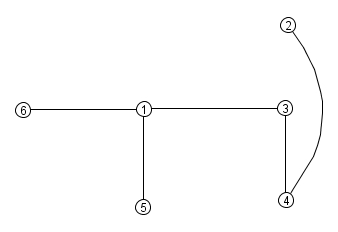
\includegraphics[width=5.5cm]{grafos_yed/g_2.jpg}
    \caption{Representa��o geom�trica (ou diagrama) do grafo $G$.}
    \label{fig:g_2}
\end{figure}

Defini-se como \textbf{v�rtices vizinhos} os v�rtices que est�o conectados as mesmas arestas que o v�rtice em quest�o:

$$ N_G(u) = \{w \in V(G) \therefore uw \in E(G)\}$$

Ou seja, para descobrir os v�rtices vizinhos (vizinhan�a) de um v�rtice $u$ verifica-se se existe um v�rtice $w$ que pertence ao conjunto de v�rtices de $G$ tal que a aresta identificada por $uw$ perten�a ao conjunto de arestas de $G$.

\paragraph*{Exemplo 2:} Para exemplificar a identifica��o da vizinhan�a, utiliza-se o v�rtice $1$ da Figura \ref{fig:g_2}:

\begin{eqnarray*}
    N_G(u) &=& N_G(1) \\
    N_G(1) &=& \{6,5,3\}
\end{eqnarray*}

O \textbf{grau de um v�rtice} (denotado por $d_G(u)$) � obtido pelo tamanho do conjunto de sua vizinhan�a, no exemplo:

\begin{eqnarray*}
    d_G(1) &=& |N(1)| \\
    d_G(1) &=& 3
\end{eqnarray*}

Defini-se como \textbf{arestas vizinhas} as arestas que incidem no v�rtice em quest�o:

$$ E_G(u) = \{e \in E(G) \therefore u \in e\} $$

Ou seja, para identificar as arestas vizinhas de um v�rtice $u$ verifica-se se uma aresta $e$ pertence ao conjunto de arestas de $G$ tal que o v�rtice $u$ esteja no conjunto de arestas $e$ em quest�o.

\paragraph*{Exemplo 3:} Para exemplificar a identifica��o das arestas vizinhas, utiliza-se o v�rtices $1$ da Figura \ref{fig:g_2}:

\begin{eqnarray*}
    E_G(u)   &=& E_G(1) \\
    E_G(1)   &=& \{\{1,6\},\{1,5\},\{1,3\}\}
\end{eqnarray*}

\subsection{Vetor de Graus}

Um vetor de grau de um grafo, � um vetor contendo os graus de todos os v�rtices do grafo.

O tamanho do vetor de graus � tamb�m o n�mero de v�rtices do grafo, no exemplo da Figura \ref{fig:g_2}, o vetor de grau � dado por:

$$ vet_G = \{1,1,1,2,2,3\}$$

Pois existem $3$ v�rtices com grau $1$, $2$ v�rtices com grau $2$ e $1$ v�rtices com grau $3$.

Sua nota��o formal � obtida por:

$$ d_G(u) \therefore u \in V(G)  $$

Ainda � poss�vel identificar se um vetor de graus � ou n�o um grafo:

\begin{itemize}
    \item � um grafo se a somat�ria dos graus de valor �mpar � par (Teorema \ref{teo:1});
    \item n�o � um grafo se o maior grau do vetor de graus � igual ou maior que o tamanho do vetor de graus.
\end{itemize}

\subsection{Grau M�nimo}

Para achar o \textbf{grau m�nimo} (denotado por $\delta$) em um grafo, deve-se identificar o menor grau do seu vetor de graus.

Dado o grafo da Figura \ref{fig:g_2}, temos:

\begin{eqnarray*}
    \delta(G) &=& min\{1,1,1,2,2,3\} \\
    \delta(G) &=& 1
\end{eqnarray*}

Definindo-se formalmente, temos:

$$ \delta(G) = min\{d_g(u) \therefore u \in V(G) \} $$

\subsection{Grau M�ximo}

Para achar o \textbf{grau m�ximo} (denotado por $\Delta$) em um grafo, deve-se identificar o maior grau do seu vetor de graus.

Dado o grafo da Figura \ref{fig:g_2}, temos:

\begin{eqnarray*}
    \Delta(G) &=& max\{1,1,1,2,2,3\} \\
    \Delta(G) &=& 3
\end{eqnarray*}

Definindo-se formalmente, temos:

$$ \Delta(G) = max\{d_g(u) \therefore u \in V(G) \} $$

\subsection{Grau M�dio}

Para achar o \textbf{grau m�dio} (denotado por $d$) em um grafo $G$ determina-se $\displaystyle\frac{1}{|V(G)|}$ (1 sobre a quantidade de v�rtices) vezes o somat�rio de todos os graus do vetor de graus ($\displaystyle\sum\limits_{u \in V(G)} d_g(u)$).

Formalmente, temos:

$$ d(G) = \frac{1}{|V(G)|} \sum\limits_{u \in V(G)} d_g(u) $$

No exemplo da Figura \ref{fig:g_2}, temos:

\begin{eqnarray*}
    d(G) &=& \frac{1}{6} \sum\limits_{u \in V(G)} d_g(u) \\
    d(G) &=& \frac{1}{6} (8) \\
    d(G) &=& \frac{8}{6} \therefore \frac{4}{3}
\end{eqnarray*}

Outra forma mais simples para achar o \emph{grau m�dio} � somar os graus do vetor de graus e dividir pelo tamanho do vetor de graus.

\subsection{Grafo n-regular}

Um grafo $G$ � dito n-regular, para um $n \in \mathbb{N}$ se todos seus v�rtices t�m grau igual a $n$.

\section{Teorema da Soma dos Graus}
\label{teo:1}

$$ \sum\limits_{u \in V} d_g(u) = 2|E(G)| $$

Prove que o somat�rio dos graus de um v�rtice do grafo $G$ com $u \in V(G)$ � igual a 2 vezes o tamanho das arestas de $G$.

Para entender melhor esse teorema vamos usar o seguinte grafo:

\begin{eqnarray*}
    G_t &=& (V(G_t), E(G_t)) \\
    V(G_t) &=& \{1,2,3,4,5\} \\
    E(G_t) &=& \{\{1,4\}, \{1,3\}, \{4,3\}, \{3,5\}, \{3,2\}\}
\end{eqnarray*}

\begin{figure}[!htb]
    \centering
    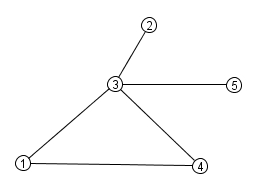
\includegraphics[width=4.5cm]{grafos_yed/g_3.jpg}
    \caption{Representa��o geom�trica (ou diagrama) do grafo $G_t$.}
    \label{fig:g_3}
\end{figure}

Analisando o teorema temos que o somat�rio dos graus do v�rtice deve ser igual a $2$ vezes o n�mero de arestas do grafo. No caso o somat�rio dos graus do v�rtice � $\sum\limits_{u \in V} d_g(u)= 10$ e o n�mero de arestas � $5$, ent�o $10 = 2(5)$.

Para cada aresta $e \in E(G)$ removida do grafo, consequentemente remove-se a liga��o entre dois v�rtices, o que diminui $2$ graus no grafo todo, logo podemos identificar uma rela��o de $2$ para $1$ (dois graus para uma aresta) entre as arestas e graus. O que confirma o teorema.

\paragraph*{Demonstra��o:} Seja $(V,E)$ um grafo, podemos definir o conjunto $X = \{(u,e) \in V x E \therefore u \in e\}$. O conjunto $X$ � um conjunto de um v�rtice $u$ ligado a uma aresta $e$ tal que esse v�rtice pertence a essa aresta. Ainda poder�amos pensar que o conjunto $X$, por um momento, relaxa as defini��es de grafos e duplica as arestas para que cada v�rtice seja separado do grafo no conjunto $X$, e leve consigo as arestas a ele conectadas. Podemos contar os elementos de $X$ de duas formas:

\begin{enumerate}
    \item \label{teo:1_1} Cada v�rtice $u$ participa de $d_g(u)$ dos elementos de $X$, portanto podemos deduzir que o tamanho de $X$ ($|X|$) � o mesmo que o somat�rio dos graus do grafo, ou formalmente $$ |X| = \sum\limits_{u \in V} d_g(u) $$
    \item \label{teo:1_2} Cada aresta $e$ est� presente em dois elementos de $X$, logo: $|X| = 2|E(G)|$.
\end{enumerate}

De \ref{teo:1_1} e \ref{teo:1_2} provamos o Teorema na Se��o \ref{teo:1}.

\subsection{Corol�rio dos Graus} \label{corolario:1}

Em todo grafo o n�mero de v�rtices com grau �mpar � par.

\paragraph*{Demonstra��o:}Seja $G$ um grafo, denote por $I$ o subconjunto formado pelos v�rtices em $V(G)$ de grau �mpar e denote por $P$ o subconjunto dos v�rtices de grau par.

\begin{eqnarray*}
    I &=& \{v \in V(G) \therefore d_g (v)\mbox{ impar}\} \\
    P &=& \{v \in V(G) \therefore d_g (v)\mbox{ par}\} \\
\end{eqnarray*}

Usando que $I \cap P = \varnothing$ e $I \cup P = V(G)$, e o Teorema da Se��o \ref{teo:1} temos:

\begin{eqnarray*}
    \sum\limits_{u \in V(G)} d_g(u) = 2|E(G)| \\
    \sum\limits_{u \in I} d_g(u) + \underbrace{\sum\limits_{u \in P} d_g(u)}_{par} = \underbrace{2|E(G)|}_{par} \\
\end{eqnarray*}

Portanto devemos ter $ \displaystyle\sum\limits_{u \in I} d_g(u) $ par, o que somente � poss�vel quando o tamanho de $I$ ($|I|$) � par.

Entretanto podemos avan�ar um pouco mais na demonstra��o e definir:

\begin{itemize}
    \item Temos um n�mero $n$ qualquer \emph{par} se definido como $n = 2k$;
    \item Temos um n�mero $n$ qualquer \emph{�mpar} se definido como $n = 2k+1$.
\end{itemize}

$$ \sum\limits_{u \in I} d_g(u) = \sum\limits_{u \in I} (2kv + 1) $$

Ent�o,

$$ \underbrace{2|E(G)|}_{par} = \biggl(\underbrace{\sum\limits_{u \in I} 2kv}_{par} + \sum\limits_{u \in I} 1 \biggl) + \underbrace{\sum\limits_{u \in P} d_g(u)}_{par}$$

Logo, o tamanho do resto do subconjunto dos \emph{�mpares} ($|I|$) deve ser \emph{par}.

    %%%%%%%%%%%%%%%%%%%%%%%
% C A P � T U L O   2 %
%%%%%%%%%%%%%%%%%%%%%%%

\chapter{Subgrafos}

Um subgrafo de um grafo $G$ � um grafo $H$ tal que:

\begin{itemize}
    \item $V(H) \subseteq V(G)$
    \item $E(H) \subseteq E(G)$
    \item $H$ deve ser um grafo
\end{itemize}

Seja um grafo $G$ definido por:

\begin{eqnarray*}
    G_c &=& (V(G_c), E(G_c)) \\
    V(G_c) &=& \{1,2,3,4\} \\
    E(G_c) &=& \{\{1,2\}, \{2,3\}, \{3,4\}, \{4,1\}\}
\end{eqnarray*}

Representado graficamente por pela Figura \ref{fig:g_4}.

\begin{figure}[!htb]
    \centering
    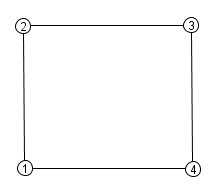
\includegraphics[width=4cm]{grafos_yed/g_4.jpg}
    \caption{Representa��o geom�trica (ou diagrama) do grafo $G_c$.}
    \label{fig:g_4}
\end{figure}

S�o representa��es de subgrafos?

\begin{enumerate}
    \item   \label{sub:1} $V(H_c) = \{1,2,3\} \\ E(H_c) = \{\{3,4\},\{1,2\}\}$ \\
	    O elemento \ref{sub:1} n�o � um subgrafo de $G_c$, pois a aresta $\{3,4\}$ cont�m um v�rtice n�o definido no conjunto de v�rtices dado, ou seja, n�o � um grafo.
    \item   \label{sub:2} $V(H_c) = \{1,2,3\} \\ E(H_c) = \{\{1,2\}\}$ \\
	    O elemento \ref{sub:2} � um subgrafo de $G_c$.
    \item   \label{sub:3} $V(H_c) = \{1,2,3,4\} \\ E(H_c) = \{\varnothing\}$ \\
	    O elemento \ref{sub:3} � um subgrafo de $G_c$.
    \item   \label{sub:4} $V(H_c) = \{1,2,3,4\} \\ E(H_c) = \{\{1,3\}\}$ \\
	    O elemento \ref{sub:4} n�o � um subgrafo de $G_c$, pois a aresta definida n�o existe no grafo original, ou seja, n�o � um grafo.
\end{enumerate}

\section{Subgrafo Gerador}

$H$ � um subgrafo gerador de $G$ se $H$ � um subgrafo de $G$ e $V(H) = V(G)$. A restri��o para um subgrafo ser gerador de algum grafo � que ele deve possuir os mesmos v�rtices do grafo original.

Por exemplo, a Figura \ref{fig:g_7} mostra dois grafos $G$ e $H$, no qual $H$ � gerador de $G$.

\begin{figure}[!htb]
    \centering
    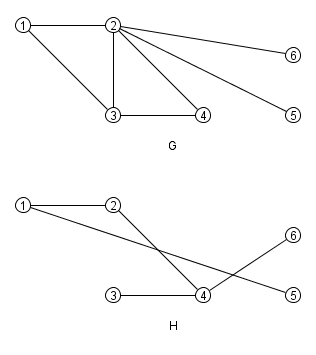
\includegraphics[width=5cm]{grafos_yed/g_7.jpg}
    \caption{$H$ � um subgrafo gerador de $G$.}
    \label{fig:g_7}
\end{figure}

Note que o grafo $H$ possui todos os v�rtices de $G$, entretanto n�o possui as mesmas arestas.

\section{Subgrafo Induzido}

Um subgrafo induzido $H$ � um subgrafo de um grafo $G$, no qual a partir de um conjunto de v�rtices ou arestas pertencentes ao grafo original $G$, � poss�vel se obter sua indu��o, denotada por $G[K]$, onde $K$ � o conjunto de arestas ou v�rtices que servir� para a indu��o.

\subsection{Por um Conjunto de V�rtices}

Um subgrafo induzido por um conjunto de v�rtices de $G$ � um subgrafo $G[S]$ de $G$ tal que:

\begin{eqnarray*}
    S &\subseteq& V(G) \\
    G[S] &=& (S,E')\\
    E'   &=& \{e \in E(G) \therefore e \subseteq S\} \mbox{ ou}\\
    E'   &=& \{e \in E(G) \therefore e \in \binom{S}{2}\} \mbox{ ou}\\
    E'   &=& E(G)\cap\binom{S}{2}
\end{eqnarray*}

As tr�s defini��es de $E'$ representam todas as arestas poss�veis em $S$ que pertencem a $E(G)$.

Em um subgrafo induzido por um conjunto de v�rtices, seu conjunto de v�rtices (V(G[S]) passa a ser o pr�prio conjunto dado, ou seja $S$. O seu conjunto de arestas � formado por todas as arestas poss�veis que interligam os v�rtices de $S$, desde que elas tamb�m estejam no grafo original $G$.

Para exemplificar, a extra��o de um subgrafo induzido por um conjunto de v�rtices � dado um grafo $G$, composto por:

\begin{eqnarray*}
    G &=& (V,E)\\
    V &=& \{1,2,3,4,5,6\}\\
    E &=& \{\{1,6\},\{1,2\},\{2,5\},\{2,4\},\{2,3\}\\
	  &&\{5,6\}\}
\end{eqnarray*}

Representado graficamente pela Figura \ref{fig:g_8}

\begin{figure}[!htb]
    \centering
    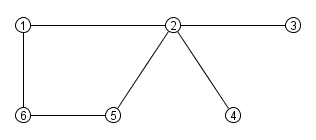
\includegraphics[width=5cm]{grafos_yed/g_8.jpg}
    \caption{Representa��o gr�fica do grafo $G$.}
    \label{fig:g_8}
\end{figure}

\paragraph*{Demonstra��o:} Obtenha o grafo induzido $G[S]$ com $S=\{1,2,5,6\}$.

Devemos ent�o copiar os v�rtices passados pelo conjunto $S$ e ent�o ligar todas as arestas poss�veis que tamb�m est�o em $G$. E assim obtemos o grafo $G[S]$ representado pela Figura \ref{fig:g_9}.

\begin{figure}[!htb]
    \centering
    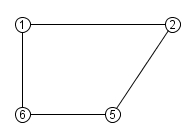
\includegraphics[width=3cm]{grafos_yed/g_9.jpg}
    \caption{Representa��o gr�fica do grafo $G[S]$.}
    \label{fig:g_9}
\end{figure}

Sua representa��o formal � dada por:

\begin{eqnarray*}
    G[S] &=& (V_s,E_s)\\
    V_s  &=& \{1,2,5,6\}\\
    E_s  &=& \{e \in E(G) \therefore e \subseteq S\}\\
    E_s  &=& \{\{1,6\},\{1,2\},\{2,5\},\{5,6\}\}
\end{eqnarray*}

\subsection{Por um Conjunto de Arestas}

Um subgrafo induzido por um conjunto de arestas $M$ de $G$ � um subgrafo $G[M]$ de $G$ tal que:

\begin{eqnarray*}
    M &\subseteq& E(G) \\
    G[M] &=& (V',M)\\
    V'   &=& \bigcup_{e \in M}e\\
\end{eqnarray*}

Em um subgrafo induzido pelo conjunto de arestas seu conjunto de arestas (E(G[M]) passa a ser o pr�prio conjunto dado, ou seja $M$. O seu conjunto de v�rtices � formado pela uni�o exclusiva do seu conjunto de arestas, o que resulta em um conjunto com todos os v�rtices necess�rios para as liga��es entre as arestas passadas como par�metro.

\paragraph*{Demonstra��o:} Utilizando o exemplo da Figura \ref{fig:g_8}, obtenha o grafo induzido $G[M]$ com $M=\{\{1,2\},\{2,5\},\{1,6\}\}$.

Devemos ent�o verificar o que resulta de $\displaystyle\bigcup_{e \in M}e$.

Obtemos ent�o o conjunto $V'=\{1,2,5,6\}$, sua representa��o gr�fica est� na Figura \ref{fig:g_10}

\begin{figure}[!htb]
    \centering
    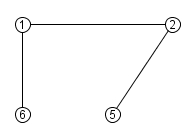
\includegraphics[width=3cm]{grafos_yed/g_10.jpg}
    \caption{Representa��o gr�fica do grafo $G[M]$.}
    \label{fig:g_10}
\end{figure}

    %%%%%%%%%%%%%%%%%%%%%%%
% C A P � T U L O   3 %
%%%%%%%%%%%%%%%%%%%%%%%

\chapter{Propriedades dos Grafos}


\section{Clique}

Em um grafo, podemos encontrar pequenos subgrafos que formam grafos completos (que s�o chamados de cliques em $G$).

Um subconjunto de v�rtices de um grafo $G$, denotado por $U$ � uma \textbf{clique} de $G$ se $G[U]$ � um grafo completo.

Em um mesmo grafo, podemos encontrar cliques de diferentes \emph{ordens}, pois podem existir diferentes subgrafos que podem ser induzidos de $G$ tal que formem um subgrafo completo.

O \textbf{tamanho da clique} � denotado pelo tamanho do conjunto de v�rtices que formam o subgrafo induzido de um determinado $G$.

Para exemplificar vamos analisar o grafo da Figura \ref{fig:g_11}

\begin{figure}[!htb]
    \centering
    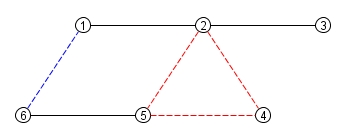
\includegraphics[width=5.5cm]{grafos_yed/g_11.jpg}
    \caption{Representa��o gr�fica do grafo $G[M]$.}
    \label{fig:g_11}
\end{figure}

No grafo da Figura \ref{fig:g_11} podemos observar dois destaques, a aresta $\{1,6\}$ (destaca em azul e pontilhado) forma uma clique de tamanho 2. Isso pois se analisarmos o subgrafo induzido por v�rtices $G[S]$, com $S=\{1,6\}$ ele � um grafo completo. Outras cliques de tamanho 2 tamb�m est�o presentes no grafo. O destaque em vermelho e pontilhado denota uma clique de tamanho 3, pois se analisarmos o subgrafo induzido por v�rtices $G[S]$, com $S=\{2,4,5\}$ ele � tamb�m um grafo completo.

\section{Conjunto Independente}

O conjunto independente pode ser definido com o oposto de uma clique em um grafo $G$ qualquer.

Dado um grafo $G$, e $U$ um conjunto de v�rtices de $V(G)$, $U$ � dito conjunto independente se $G[U] = (V, \varnothing)$.

Ou seja, um subconunto de v�rtices que n�o possui liga��o de uma aresta entre eles.

Para exemplificar um conjunto independente podemos analisar o grafo da Figura \ref{fig:g_20}

\begin{figure}[!htb]
    \centering
    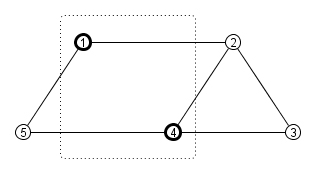
\includegraphics[width=5cm]{grafos_yed/g_20.jpg}
    \caption{Conjunto independe $U$ no grafo $G$}
    \label{fig:g_20}
\end{figure}

O conjunto $U$ � dado por:

\begin{eqnarray*}
    U &=& \{1,4\}
\end{eqnarray*}

Assim como na clique o tamanho ou ordem do conjunto independente � dado pelo tamanho do conjunto de v�rtices do subgrafo induzido que forma o conjunto independente.

\subsection{Teorema da Clique e Conjunto Independente M�ximos} \label{teo:2}

Seja:

\begin{eqnarray*}
    \omega(G) &=& \mbox{max}\{|A| \therefore A \subseteq V(G) \mbox{ e } A \mbox{ � clique}\\
    \alpha(G) &=& \mbox{max}\{|A| \therefore A \subseteq V(G) \mbox{ e } A \mbox{ � um conj. indep.}\\
\end{eqnarray*}

\begin{center}
    Prove que $\omega(G) = \alpha(\overline{G})$.
\end{center}

\paragraph*{Prova:} Seja $S$ uma clique de $G$ com $|S| = \omega(G)$. Logo $G[S] = (S, \displaystyle\binom{S}{2})$.

Em $\overline{G}$ uma aresta que pertence a $G$ � uma aresta se e somente se n�o pertence a $E(G)$. Logo, ($e \in E(\overline{G}) \Leftrightarrow \not\in E(G)$). Se $S$ � uma clique em $G$, em seu grafo complementar $\overline{G}$, $S$ ser� um conjunto independente. Logo, $\overline{G}[S] = (S, \varnothing)$.

Como $\omega(G) = |S|$ e $\alpha(\overline{G}) \geqslant S$. Ou seja o tamanho do conjunto $S$ criado � o tamanho da clique m�xima encontrada em $G$ e como essa clique � um conjunto independente em $\overline{G}$, ent�o existe pelo menos um conjunto independente em $\overline{G}$ do mesmo tamanho ou maior que $S$.

Logo, $\omega(G) \leqslant \alpha(\overline{G})$.

Seja $U$ um conjunto independente em $\overline{G}$ com $|U| = \alpha(\overline{G})$. Logo $\overline{G}[U] = (U, \varnothing)$.

Logo $G[U] = (U, \displaystyle\binom{U}{2})$.

Em $G$ uma aresta que pertence a $\overline{G}$ � uma aresta se e somente se n�o pertence a $E(\overline{G})$. Logo, ($e \in E(G) \Leftrightarrow \not\in E(\overline{G})$). Se $U$ � um conjunto independente em $G$, em seu grafo complementar $\overline{G}$, $U$ ser� uma clique.

Como $\alpha(\overline{G}) = |U|$ e $\omega(G) \geqslant |U|$. Logo $\omega(G) \geqslant \alpha(\overline{G})$.

Ent�o, como:

\begin{eqnarray*}
    \omega(G) &\geqslant& \alpha(\overline{G}) \mbox{ e}\\
    \omega(G) &\leqslant& \alpha(\overline{G}) \mbox{ ent�o}\\
    \omega(G) &=& \alpha(\overline{G})
\end{eqnarray*}

\section{Grafo Bipartido}

Um grafo $G$ � bipartido se existem dois conjuntos independentes $A$ e $B$ em $G$ que particionam $V(G)$, ou seja $A \cup B = V(G)$ e $A \cap B = \varnothing$.

\paragraph*{Exemplo 4:}Para exemplificar o conceito de grafo bipartido, vamos analisar o grafo da Figura \ref{fig:g_21}.

\begin{figure}[!htb]
    \centering
    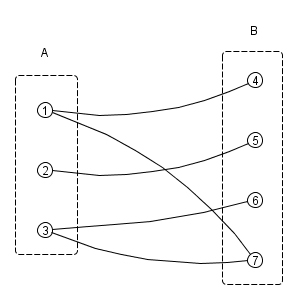
\includegraphics[width=5cm]{grafos_yed/g_21.jpg}
    \caption{Exemplo de Grafo Bipartido.}
    \label{fig:g_21}
\end{figure}

� poss�vel identificar dois conjuntos no grafo, os elementos do conjunto $A$ s�o $V(A) = \{1,2,3\}$ e apenas se interligam com os elementos do conjunto $B$ dado por $V(B) = \{4,5,6,7\}$.


O Algoritmo \ref{alg:1} mostra um algoritmo para achar dois conjuntos $A$ e $B$ em um grafo bipartido.

%    \begin{table*}
%    \texttt{\lstinputlisting[language=C, label=alg:bipartido,
%    caption={Algoritmo para encontrar dois conjuntos $A$ e $B$ em um grafo bipartido.}]{cods/alg_bipartido.txt}}
%    \end{table*}

\begin{algorithm}
    \small{
    \SetAlgoNoEnd
    $Bipartido(G)$\;
    \Inicio{
	$A[] \leftarrow $ lista vazia de v�rtices\;
	$B[] \leftarrow $ lista vazia de v�rtices\;
	$u \leftarrow $v�rtice aleat�rio de $V(G)$\;
	\Enqto{$u$ n�o for o �ltimo v�rtice de $V(G)$}{
	    \Se{$N_G(u)$ est� em $A$ e $N_G(u)$ est� em $B$}{
		o grafo $G$ n�o � bipartido\;
	    }
	    \eSe{$N_G(u)$ est� em $A$}{
		adicione $u$ em $B$\;
	    }{
		adicione $u$ em $A$\;
	    }
	    $u \leftarrow$ o pr�ximo v�rtice vizinho n�o visitado de $u \in V(G)$\;
	}
    }
    \caption{Verifica se $G$ � bipartido ou n�o}
    \label{alg:1}
    }
\end{algorithm}

No Algoritmo \ref{alg:1}, criamos duas listas de v�rtices $A$ e $B$ que ser�o os conjuntos que no final da execu��o conter�o os elementos que n�o se conectam. Inicialmente se escolher um $u$ qualquer, e para todo $u$ do conjunto de v�rtices se verifica se algum de seus vizinhos est� no grupo $A$, se estiver ele � colocado em $B$, caso contr�rio em $A$.

\paragraph*{Exemplo 5:}O seguinte $G$ � definido por:

\begin{eqnarray*}
    V(G) &=& \{1,2,3,4,5,6,7,8\}\\
    E(G) &=& \{\{1,6\},\{6,2\},\{3,7\},\{3,8\},\{7,4\},\\
	      &&\{7,5\}\}
\end{eqnarray*}

� bipartido, pois $V(G) = A \cup B$ e $V(A) = \{1,2,3,4\}$ e $V(B) = {6,7,8}$ e tanto $A$, como $B$ s�o conjuntos independentes.

No mesmo grafo ainda � poss�vel identificar outros conjuntos que deixam o grafo bipartido. Seja $A'$ e $B'$, se $V(A') = \{1,2,7,6\}$ e $V(B') = \{2,3,5,4\}$ ent�o $A'$ e $B'$ formam conjuntos independentes.

Um grafo pode ser bipartido formando diferentes conjuntos independentes. Como pode ser observado com os conjuntos $A$ e $B$ e $A'$ e $B'$.

\subsection{Subgrafo Bipartido Completo}

Um grafo bipartido $G$ com partes $A$ e $B$ � dito \textbf{completo} se tem $|A| \cdot |B|$ arestas. ou seja, $E(G) = \{\{a,b\} \subseteq V(G) \therefore a \in A \mbox{ e } b \in B$. Um grafo bipartido completo com partes de cardinalidade $n$ e $m$ � denotado por $K^{n,m}$.

Todos os elementos do conjunto $A$ devem se ligar a todos elementos do conjunto $B$ e vice versa, como podemos observar no grafo da Figura \ref{fig:g_26}.

\begin{figure}[!htb]
    \centering
    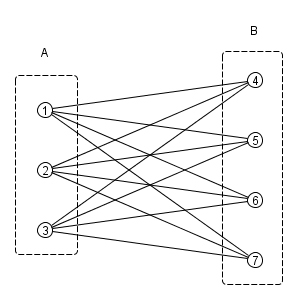
\includegraphics[width=5cm]{grafos_yed/g_26.jpg}
    \caption{Exemplo de Grafo Bipartido Completo.}
    \label{fig:g_26}
\end{figure}

No grafo de exemplo da Figura \ref{fig:g_26}, podemos representar esse subgrafo bipartido completo por $K^{n,m}$.

\section{Corte}

Um corte � um conjunto de arestas que "separam"{} dois conjuntos de v�rtices.

Dados $A,B \subseteq V(G)$ e $A \cap B = \varnothing$. Ent�o, $E(A,B) = \{\{u,v\} \in E(G) \therefore u \in A \mbox{ e } v \in B\}$.

Para exemplificar o conceito de corte vamos usar o grafo $G$ da Figura \ref{fig:g_22}.

\begin{figure}[!htb]
    \centering
    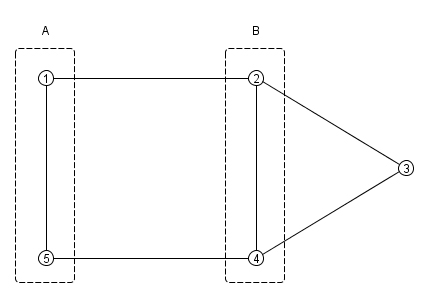
\includegraphics[width=6.5cm]{grafos_yed/g_22.jpg}
    \caption{Exemplo de Corte em um Grafo.}
    \label{fig:g_22}
\end{figure}

Ent�o o corte $E(A,B)$ para o grafo $G$ indicado na Figura \ref{fig:g_22}, � dado por: $E(A,B) = \{\{1,2\}, \{5,4\}\}$.

Para identificar um corte em um grafo $G$ definido por:

\begin{eqnarray*}
    V(G) &=& \{1,2,3,4,5\}\\
    E(G) &=& \{\{1,2\},\{2,5\},\{5,4\},\{4,3\},\{4,2\}\\
	      &&\{1,5\}\}
\end{eqnarray*}

podemos seguir 2 passos:

\begin{enumerate}
    \item Identificar 2 conjuntos de v�rtices tais que, se um conjunto for o conjunto $T \subseteq V(G)$, ent�o $\overline{T} = V(G) \smallsetminus T$;
    \item Verificar se existem uma ou mais arestas que ligam os elementos do conjunto $T$ com o conjunto $\overline{T}$.
\end{enumerate}

Sejam dois conjuntos $T$ e $\overline{T}$ dados por:

\begin{eqnarray*}
    T &=& \{1,2\}\\
    \overline{T} &=& \{3,4,5\}
\end{eqnarray*}

Ent�o, um corte do tipo $E(T,\overline{T}) = \{u,v\} \subseteq V(G) \therefore u \in T e v \in \overline{T})$ ou seja, $E(T,\overline{T}) = \{\{3,1\},\{2,4\},\{2,5\}\}$.

O grafo $G$ e os cortes (destacados em pontilhado) podem ser observados na Figura \ref{fig:g_28}

\begin{figure}[!htb]
    \centering
    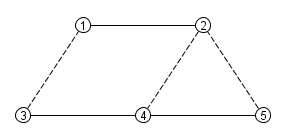
\includegraphics[width=5cm]{grafos_yed/g_28.jpg}
    \caption{Outro Exemplo de Corte em um Grafo.}
    \label{fig:g_28}
\end{figure}

\paragraph*{Observa��o:} Os cortes interessantes s�o do tipo $E(S, \overline{S})$.

Com o conceito de corte, podemos definir um \textbf{grafo bipartido} de outra nova maneira:

$G$ � um grafo bipartido se existe $S \subset V(G)$ n�o vazio tal que $E(G) = E(S, \overline{S})$ e n�o exista arestas entre $S$ e $\overline{S}$.

\section{Isomorfismo}

Dizemos que os grafos $G$ e $H$ s�o \textbf{isomorfos}, e nesse caso escrevemos $G \simeq H$, se existe uma fun��o bijetora.

Uma fun��o bijetora garante que cada elemento do conjunto $A$ vai possuir um elemento \textbf{correspondente} no conjunto $B$.

$$ f: V(G) \rightarrow V(H)$$

tal que,

$$ \{u,v\} \in E(G) \Leftrightarrow \{f(u),f(v)\} \in E(H) $$

Para que dois grafos sejam isomorfos, devem ter:

\begin{itemize}
    \item o mesmo tamanho de arestas;
    \item o mesmo tamanho de v�rtices;
    \item o mesmo vetor de graus;
    \item uma fun��o bijetora do tipo $f: V(G_1) \rightarrow V(H)$.
\end{itemize}

\paragraph*{Exemplo 6:} Sejam $G_1$, $G_2$ e $G_3$ os grafos definidos por:

\begin{eqnarray*}
    V(G_1) &=& \{1,2,3,4,5,6\}\\
    V(G_2) &=& V(G_1)\\
    V(G_3) &=& V(G_2)\\
    E(G_1) &=& \{\{1,2\}, \{2,3\}, \{3,4\}, \{4,5\}, \{5,6\},\\
	    & &   \{6,1\}\}\\
    E(G_2) &=& \{\{1,3\}, \{3,5\}, \{5,1\}, \{2,4\}, \{4,6\},\\
	    & &   \{6,2\}\}\\
    E(G_3) &=& \{\{1,3\}, \{3,5\}, \{5,6\}, \{6,2\}, \{2,4\},\\
	    & &   \{4,1\}\}\\
\end{eqnarray*}

e dispostos na Figura \ref{fig:g_27}.

\begin{figure}[!htb]
    \centering
    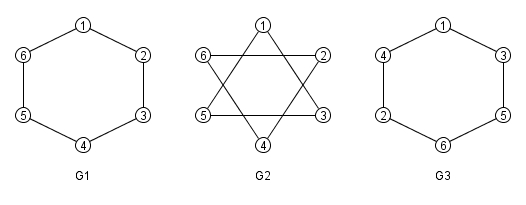
\includegraphics[width=8cm]{grafos_yed/g_27.jpg}
    \caption{Exemplo de Isomorfismo.}
    \label{fig:g_27}
\end{figure}

Pergunta-se, $G_1$, $G_2$ e $G_3$ s�o isomorfos entre s�?

Os grafos $G_1$ e $G_3$ s�o isomorfos, pois t�m o mesmo formato, al�m do mesmo vetor de graus, mesmo n�mero de arestas, mesmo n�mero de v�rtices e pode-se identificar a seguinte fun��o bijetora:

$$ f: V(G_1) \rightarrow V(G_3) $$

\begin{center}
\begin{tabular}{|c|c|}
  \hline
  1 & 1 \\
  \hline
  2 & 3 \\
  \hline
  3 & 5 \\
  \hline
  4 & 6 \\
  \hline
  5 & 2 \\
  \hline
  6 & 4 \\
  \hline
\end{tabular}
\end{center}

Pois se testarmos para cada aresta do grafo $G_1$ existe uma correspondente no grafo $G_3$. Por exemplo a aresta $\{1,2\}$ ao aplicarmos a fun��o se transforma na aresta $\{1,3\}$ que est� presente no conjunto de arestas de $G_3$. Para que eles sejam isomorfos, ao se aplicar a fun��o bijetora em todas as arestas de $G_1$ devemos obter uma equivalente em $G_3$.

O grafo $G_2$ n�o � isomorfo a $G_1$ ou $G_3$, pois em $G_2$, o conjunto de v�rtices $\{1,3,5\}$ forma um tri�ngulo $K_3$ que n�o est� presente em $G_1$ ou $G_3$.

Grafos isomorfos entre si possuem o mesmo desenho (visualmente), entretanto a localiza��o dos v�rtices podem ser diferentes como � poss�vel observar em $G_1$ e $G_3$. Grafos s�o quase iguais, o que os torna diferentes � o nome dado aos seus v�rtices.

Para montar a tabela da fun��o bijetora, devemos testar todas as combina��es poss�veis entre os v�rtices dos grafos dados. Para um grafo com um n�mero expressivo de v�rtices, uma alternativa mais eficiente �:

\begin{itemize}
    \item identificar e separar v�rtices do mesmo grau nos dois grafos;
    \item fazer a permuta��o entre esses v�rtices;
    \item testar as combina��es entre todas as permuta��es dos graus.
\end{itemize}

Outra defini��o para \textbf{isomorfismo} � que dois grafos $G$ e $H$ s�o isomorfos se existe um \textbf{isomorfismo} entre eles. Em outras palavras, dois grafos s�o isomorfos se � poss�vel alterar os nomes dos v�rtices de um deles de tal modo que os dois grafos fiquem iguais.

Para decidir se dois grafos $G$ e $H$ s�o isomorfos, basta examinar todas as bije��es de $V(G)$ em $V(H)$. Se cada um dos grafos tem $n$ v�rtices, esse algoritmo consome tempo proporcional a $n!$. Como $n!$ cresce explosivamente com $n$, esse algoritmo � decididamente insatisfat�rio na pr�tica. Infelizmente, n�o se conhece um algoritmo substancialmente melhor.

\section{Outras No��es de Grafos}

Em algumas situa��es podemos ter um modelo para um problema a ser resolvido e esse modelo seria um grafo se desconsiderassemos algumas peculiaridades da situa��o. Por exemplo, um mapa rodovi�rio pode ser modelado definindo-se um v�rtice para cada cidade e duas cidades formam uma aresta no grafo (modelo) se existe rodovia ligando essas cidades correspondentes aos v�rtices. Normalmente, dist�ncia � um par�metro importante nesses mapas e assim as arestas devem ter um comprimento associado a elas.

Entretanto, "comprimento de aresta"{} n�o faz parte da defini��o de um grafo. Num outro exemplo, se estamos interessados em rotas de tr�fego dentro de uma cidade podemos definir um v�rtice por esquina e duas esquinas consecutivas numa mesma rua formam uma aresta. Nesse caso, as ruas t�m sentido (m�o e contra-m�o) e as arestas tamb�m deveriam ter mas, novamente, essa caracter�stica n�o faz parte da defini��o de grafos.

Esses problemas e muitos outros podem ser modelados com "outros tipos"{} de grafos. Alguns desses outros tipos s�o:

\begin{itemize}
    \item \textbf{Grafo com pesos nas arestas} � um tripla $(V,E,\rho)$ de modo que $(V,E)$ � um grafo e $\rho: E \rightarrow R$ � uma fun��o que assume valores em $R \subseteq \mathbb{R}$. O conjunto $R$ em geral depende do problema sendo considerado. Por exemplo, se os pesos representam dist�ncia ent�o tomamos $R + \mathbb{R}^+$ (reais n�o-negativos). O grafo $(V,E)$ � chamado grafo subjacente do grafo com pesos nas arestas;

    \item \textbf{Grafo orientado} � aquele onde as arestas t�m uma orienta��o (s�o pares ordenados) de modo que se $u$ e $v$ s�o v�rtices, ent�o $(u,v) \neq (v,u)$ e al�m disso se $(u,v)$ � uma aresta ent�o $(v,u)$ n�o � aresta. Removendo o sentido das arestas temos o grafo subjacente ao grafo orientado;

    \item \textbf{Grafos dirigido} ou digrafo � dado $(V,E)$ onde $E \subseteq V � V \smallsetminus {(v,v) \therefore v \in V }$;

    \item \textbf{Multigrafo} � dado por um conjuntode v�rtices e podemos ter mais de uma aresta incidente ao mesmo par de v�rtices. Removendo as arestas repetidas de um multigrafo temos o \textit{grafo subjacente} ao multigrafo.
\end{itemize}

\begin{figure}[!htb]
    \centering
    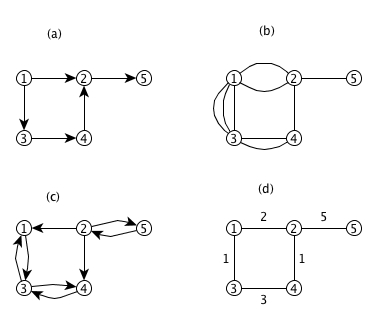
\includegraphics[width=7cm]{grafos_yed/g_32.jpg}
    \caption{(a) Grafo orientado. (b) Multigrafo. (c) Grafo dirigido. (d) Grafo subjacente}
    \label{fig:g_32}
\end{figure}

    %%%%%%%%%%%%%%%%%%%%%%%
% C A P � T U L O   4 %
%%%%%%%%%%%%%%%%%%%%%%%

\chapter{Representa��es Computacionais de Grafos}

Para representar os grafos estudados em um ambiente computacional devemos estudar qual estrutura devemos utilizar. Em geral, a estrutura de dados adotada est� relacionada com qual a fun��o do algoritmo que ir� atuar no grafo.

Em casos gerais, com uma estrutura b�sica dever�amos ser capazes de responder as perguntas:

\begin{enumerate}
    \item \label{rc:p1} qual � o tamanho do conjunto de v�rtices de um grafo $G$? $|V(G)|$
    \item \label{rc:p2} qual � o tamanho do conjunto de arestas de um grafo $G$? $|E(G)|$
    \item \label{rc:p3} qual � o grau de um determinado v�rtice de um grafo $G$? $d_G(u) \therefore u \in V(G)$
    \item \label{rc:p4} uma aresta $\{u,v\}$ pertence ao conjunto de arestas do grafo $G$? $\{u,v\} \in E(G)$
    \item \label{rc:p5} qual a vizinhan�a de um v�rtice $u$ do conjunto de v�rtices do grafo $G$? $N_G(u) \therefore u \in V(G)$
\end{enumerate}

Algumas perguntas, como a \ref{rc:p3}, s�o \emph{perguntas secund�rias}, por exemplo o grau de um v�rtice est� ligado com a quantidade de vizinhos desse v�rtice, outro exemplo de \emph{pergunta secund�ria} � uma pergunta do tipo: \emph{O grafo $G$ � completo?}, pois tamb�m depende de outras informa��es obtidas por perguntas prim�rias.

Para representa��o computacional de um grafo, � necess�rio trechos de algoritmos que percorram os vizinhos de um determinado v�rtice, assim respondendo tanto perguntas prim�rias quanto secund�rias.

Uma das perguntas mais recorrentes nos algoritmos que percorrem os nodos de um grafo �: "para todo $u \in N_g(v)$ fa�a"{}. Essa pergunta pode ser traduzida de duas formas diferentes:

\begin{itemize}
    \item "para todo $u \in V(G) \therefore \{u,v\} \in E$ fa�a";
    \item "$u \leftarrow$ primeiro vizinho $(v)$"{} + "$u \leftarrow$ pr�ximo vizinho $(v)$".
\end{itemize}

O primeiro la�o necessita que se responda a pergunta \ref{rc:p4}, enquanto que a segunda necessita que se responda a pergunta \ref{rc:p5}.

Uma quest�o interessante ao se codificar a estrutura de dados de um grafo � o m�todo de indexa��o, \textbf{v�rtices x arestas}. Mesmo assim existem casos particulares em que algum tipo de indexa��o pode ser mais eficiente que outro.

\section{Lista de Arestas}

� uma representa��o de um grafo na qual � dado um vetor ou lista com pares de v�rtices representando as arestas desse grafo.

\paragraph*{Exemplo 7:}
\label{rc:exemplo}

Seja um grafo $G$ de exemplo, definido por:

\begin{eqnarray*}
    V(G) &=& \{1,2,3,4,5\}\\
    E(G) &=& \{\{1,2\},\{2,5\},\{5,4\},\{4,3\},\{4,2\}\}
\end{eqnarray*}

Sua representa��o por lista de arestas � dada por:

$$ \{1,2\}, \{2,5\}, \{5,4\}, \{4,3\}, \{4,2\} $$

Para representar os v�rtices nessa nota��o utiliza-se um vetor de v�rtices de 1 a $n$ com $n = |V(G)|$.

$$ V = \{1,2,3,4,5\} $$

Com essa estrutura, responder a pergunta \ref{rc:p4} ($\{u,v\} \in E(G)$) custa $\Theta(m)$ onde $m = |E(G)|$.

Responder a pergunta \ref{rc:p5} ($N_G(u) \therefore u \in V(G)$), tamb�m tem o custo $\Theta(m)$ onde $m = |E(G)|$.

Isso porque nos dois casos � necess�rio percorrer a lista de arestas, no primeiro caso apenas verificando se $u$ e $v$ est�o na lista $E_{i,j}$. No segundo caso, procura-se por $u$, ao se achar anota-se o vizinho, e continua-se da pr�xima aresta $E_{i,j}$.

\section{Matriz de Adjac�ncias}

� uma matriz $n$ x $m$ tal que:

$$
M_{i,j} =   \left\{ \begin{array}{rll}
			0 & \mbox{se} & i,j \not\in E(G) \\
			1 & \mbox{se} & i,j \in E(G)
		    \end{array}\right.
$$

Essa matriz � sim�trica, quadrada e possui sua diagonal preenchida por $0$.

O custo para descobrir a pergunta \ref{rc:p4} ($\{u,v\} \in E(G)$) custa $\Theta(1)$. 

Responder a pergunta \ref{rc:p5} ($N_G(u) \therefore u \in V(G)$), tem o custo $\Theta(m)$ onde $m = |V(G)|$.

Segue a representa��o do Exemplo \ref{rc:exemplo} por matriz de adjac�ncias:

$$
\left(
  \begin{array}{cccccc}
    \# & 1 & 2 & 3 & 4 & 5 \\
    1  & 0 & 1 & 0 & 0 & 0 \\
    2  & 1 & 0 & 0 & 1 & 1 \\
    3  & 0 & 0 & 0 & 1 & 0 \\
    4  & 0 & 1 & 1 & 0 & 1 \\
    5  & 0 & 1 & 0 & 1 & 0 \\
  \end{array}
\right)
$$

\section{Listas de Adjac�ncia}

� um vetor de listas indexado pelos v�rtices e cada lista representa uma vizinhan�a.

Na Figura \ref{fig:g_29} podemos observar uma representa��o por lista de adjac�ncias do Exemplo \ref{rc:exemplo}.

\begin{figure}[!htb]
    \centering
    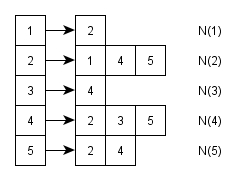
\includegraphics[width=3.7cm]{grafos_yed/g_29.jpg}
    \caption{Lista de Adjac�ncias.}
    \label{fig:g_29}
\end{figure}

Responder a pergunta \ref{rc:p5} ($N_G(u) \therefore u \in V(G)$), tem o custo $\Theta(m)$ onde $m = |N_G(u)|$.

\section{Pesos}

Para atribuir pesos aos v�rtices ou arestas, podemos utilizar:

\begin{itemize}
    \item v�rtices: criar um vetor associado.
    \item arestas:
    \begin{enumerate}
	\item criar um nome para cada aresta e criar tamb�m um vetor associado;
	\item na matriz de adjac�ncias armazenar a informa��o na c�lula $M_{i,j}$;
	\item na lista de adjac�ncias armazenar uma pequena informa��o em cada vizinho.
    \end{enumerate}
\end{itemize}

Uma boa pr�tica � a cria��o de um vetor associado para armazenar os graus de um v�rtice.

\section{Vantagens e Desvantagens}

As estruturas ilustradas apresentam vantagens e desvantagens, o que � retornado em um melhor tempo por uma estrutura n�o retornado por outra, por isso deve-se analisar o algoritmo a ser escrito, para que escolha-se a estrutura mais adequada de acordo com as opera��es que ir�o ser feitas.

A matriz de adjac�ncias, apresenta um outro problema que � o espa�o desperdi�ado quando se tem grafos espa�os (com poucas arestas), pois a matriz ir� ser preenchida por muitos espa�os vazios.

Em algumas implementa��es, pode se tornar interessante preservar as duas estruturas (matriz de adjac�ncias e listas de adjac�ncias) para se obter um melhor desempenho. A desvantagem � manter a persist�ncia em ambas estruturas, e o espa�o ocupado duplicado.


    %%%%%%%%%%%%%%%%%%%%%%%
% C A P � T U L O   5 %
%%%%%%%%%%%%%%%%%%%%%%%

\chapter{Percursos em Grafos}

Para ilustrar os estudos dos percursos vamos utilizar o grafo disposto na Figura \ref{fig:g_33}

\begin{figure}[!htb]
    \centering
    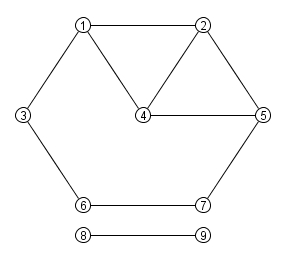
\includegraphics[width=4.5cm]{grafos_yed/g_33.jpg}
    \caption{Grafo de Exemplo para estudo de Caminhos e Circuitos.}
    \label{fig:g_33}
\end{figure}

Dado um grafo $G(V,E)$ com uma aresta ${v,w} \in V(G)$, ent�o podemos definir o conceito de \textbf{alcans�vel}:

O v�rtice $v$ � alcans�vel pelo v�rtice $w$ no grafo $G$ se existe um conjunto de v�rtices denotado por um conjunto $P$ ou seja $P(v_1, v_2, v_3, \ldots, v_n)$ tal que:

\begin{itemize}
    \item $v_i \in V(G) \mbox{ para } i \in \{1,2,3,\ldots,n\}$
	  Os v�rtices a serem percorridos est�o presentes no conjunto de v�rtices do grafo dado;
    \item $v_1 = v$
	  O primeiro v�rtice do conjunto se torna o v�rtice inicial dado, no caso $v$;
    \item $v_n = w$
	  O �ltimo v�rtice do conjunto � o v�rtice final dado, no caso $w$;
    \item $\{v_i, v_{i+1}\} \in E(G), \mbox{ para } i \in \{1,2,3,\ldots,n\}$
	  Existe uma aresta que liga o v�rtice $v_i$ com o v�rtice $v_{i+1}$ no conjunto de arestas dado.
\end{itemize}

No exemplo da Figura \ref{fig:g_33}, o v�rtice 4 � alcans�vel pelo v�rtice 6. Entretanto o v�rtice 8 n�o � alcans�vel pelo v�rtice 7.

Um \textbf{passeio} em um grafo � uma sequ�ncia de arestas do tipo $\{\{v_0,v_1\},\{v_1,v_2\}, \ldots, \{v_{s-1},v_s\}\}$ onde $s$ � o comprimento do passeio. Um passeio n�o possui um limite, � poss�vel passear pelo grafo repetindo v�rtices e arestas.

No exemplo da Figura \ref{fig:g_33}, poder�amos definir um passeio $P_1\{\{6,3\}, \{3,1\}, \{1,4\}, \{4,1\}\}$.

Um \textbf{caminho} em um grafo � um passeio que n�o possui repeti��o de v�rtices. Sua defini��o formal � dada por:

$$ v_i \neq v_j \mbox{ para } i \neq j$$

O limite de um caminho se refere a situa��o de estar em determinado v�rtice $v$ e n�o poder inserir outro vizinho $v$ por todos j� estarem contidos no caminho. Um caminho normalmente visa atingir um determinado objetivo, ou seja ir de um v�rtice para outro.

No exemplo da Figura \ref{fig:g_33}, poder�amos definir um caminho $C_1\{6,7,8,4,2\}$.

Uma \textbf{trilha} em um grafo � um passeio que n�o possui repeti��o de arestas. Sua defini��o formal � dada por:

$$ \{v_i,v_{i+1}\} \neq \{v_j,v_{j+1}\} \mbox{ para } i \neq j$$

No exemplo da Figura \ref{fig:g_33}, poder�amos definir uma trilha $C_1\{\{6,3\}, \{3,1\}, \{1,4\}, \{4,2\}\}$. Note que o v�rtice 4 foi repetido, entretanto para arestas diferentes.

A \emph{diferen�a} entre trilha e caminho � que a trilha permite repeti��o de v�rtices, desde que n�o se repitam arestas.

Uma trilha pode ser imaginada como um desenho marcado em determinado grafo, que indica um caminho marcado.

Um \textbf{circuito ou ciclo} � um caminho que come�a e acaba com o mesmo v�rtice. Ciclos de comprimento 1 s�o la�os. No grafo de exemplo, $\{1,4,5,2,1\}$ � um ciclo de comprimento 4 (o comprimento de um ciclo � dado pela contagem de arestas). Sua defini��o formal � dada por:

\begin{eqnarray*}
    v_1 &\neq& v_j, \mbox{ para } i \neq j \\
    v_1 &=& v_n
\end{eqnarray*}

A \textbf{dist�ncia} de um v�rtice $u$ a um v�rtice $w$ � o n�mero de arestas de um caminho m�nimo de $u$ a $w$. Sua defini��o formal � dada por:

$ {dist}_G(u,w) = min\{k\} $, onde $u$ e $w$ s�o extremos de um caminho de tamanho $k$.

\paragraph*{Observa��o} N�o faz sentido dizer "\emph{a menor dist�ncia}"{} ou "\emph{a dist�ncia m�nima}":  dist�ncia j� � m�nima por defini��o. Portanto, dizer que a dist�ncia de $u$ a $w$ � $k$ significa duas coisas:

\begin{enumerate}
    \item existe um caminho de $u$ a $w$ com exatamente $k$ arestas;
    \item n�o existe caminho de $u$ a $w$ com menos que $k$ arestas.
\end{enumerate}

Caso $u$ n�o seja alcans�vel por $w$ ent�o podemos dizer que a dist�ncia ${dist}_G(u,w) = \infty$.

No exemplo da Figura \ref{fig:g_33}, ${dist}_G(7,8) = \infty$ e ${dist}_G(6,1) = 2$.

%     \subsection{Teoremas}

%     \begin{enumerate}
%         \item ${dist}_G(u,v) = {dist}_G(v,u)$
%         \item ${dist}_G(u,v) = 0 \leftrightarrow u=v$
%         \item ${dist}_G(u,v) \leqslant {dist}_G(u,v) + {dist}_G(v,w)$
%         \item Dado o grafo $G=(V,E)$, existe um caminho de tamanho pelo menos $\delta(G)$ e um circuito de tamanho pelo menos $\delta(G)+1$ para $\delta(G) \geqslant 2$.
%     \end{enumerate}

\section{Algoritmo Gen�rico de Busca}

Nessa sess�o vamos estudar um algoritmo gen�rico para percorrer um grafo dado. Para isso iremos tomar como exemplo base o seguinte problema:

Dado um grafo $G$ e um v�rtice $s \in E(G)$, encontrar $S \subseteq V(G)$ tal que para todo $v \in S$ existe um caminho de $s$ a $v$.

Com um grafo e um v�rtice qualquer, devemos descobrir todos os v�rtices alcans�veis para o v�rtice passado.

\begin{itemize}
    \item visite(G,s);
    \item dado: um grafo $G$ e um v�rtice $s \in V(G)$;
    \item devole: um conjunto $S$ de v�rtices alcans�veis a partir de $s$;
\end{itemize}

O algoritmo visite(G,s) est� descrito no Algoritmo \ref{alg:2}.

\begin{algorithm}
    \small{
    \SetAlgoNoEnd
    $visite(G, s)$\;
    \Inicio{
	$L[] \leftarrow $ conjunto de v�rtices vazio\;
	$L \leftarrow s$\;
	marque $s$ como visistado e $V(G) \smallsetminus s$ como n�o-visistado\;
	marque as arestas de $E(G)$ como n�o-visistads\;
	\Enqto{$L \neq \emptyset$}{
	    escolha $v$ pertencente a $L$\;
	    \eSe{em $E_G(v)$ existe uma aresta n�o visistada a partir de $v$}{
		escolha $\{v,w\}$ em $E_G(v)$ n�o visistada a partir de $v$\;
		marque $\{v,w\}$ como visitada a partir de $v$\;
		\Se{$w$ � n�o-visistado}{
		    insista $w$ em $L$\;
		    marque $w$ como visistado\;
		}
	    }
	    {
		remova $v$ de $L$\;
	    }
	}
    }
    \caption{Algoritmo de Busca ou Percurso}
    \label{alg:2}
    }
\end{algorithm}

%    \begin{table*}
%    \texttt{\lstinputlisting[language=C, label=alg:busca,
%    caption={Algoritmo de Busca ou Percurso.}]{cods/alg_busca.txt}}
%    \end{table*}

\subsection{Custo do Algoritmo}

O n�mero de vezes que um v�rtice $u$ � escolhido como $v$ � $d_G(u)+1$. Isso por que ele � escolhido 1 vez para visistar cada aresta incidente a $u$ e uma vez para ser eliminado do conjunto $L$.

Como cada v�rtice entra no m�ximo 1 vez em $L$, o n�mero de vezes que um v�rtice � escolhido, � no m�ximo $\displaystyle\sum_{v \in S}|d_G(v)+1|$.

\begin{eqnarray*}
    \sum_{v \in S}|d_G(v)+1| &=& \sum_{v \in S}|d_G(v)| + \sum_{v \in S}|1|\\
    &=& 2|E(G[S])| + |S| \leqslant 2m + n
\end{eqnarray*}

A complexidade de tempo do algoritmo visite(G,s) � $\Theta(2|E(G[S])| + |S|)$ ou $\Theta(m+n)$, como $m$ sendo o n�mero de arestas e $n$ sendo o n�mero de v�rtices.

\section{Tipo de Busca}

A forma como a estrutura de dados ser� implementada indica o tipo de busca que ser� efetuada, se a estrutura que armazena $L$ for implementada em uma pilha, ent�o a busca se dar� em profundidade:

\begin{itemize}
    \item o algoritmo come�a pelo n� raiz e explora tanto quanto poss�vel cada um dos seus ramos, antes de retroceder (\emph{backtracking});
\end{itemize}

  caso a estrutura que armazena $L$ seja implementada como uma fila, ent�o a busca se dar� em largura:

\begin{itemize}
    \item o algoritmo come�a pelo n� raiz e explora todos os n�s vizinhos; ent�o, para cada um desses n�s mais pr�ximos, explora-se os seus n�s vizinhos inexplorados e assim por diante.
\end{itemize}

\subsection{Busca em Profundidade}

Esse tipo de busca usar um percurso utilizando uma pilha como estrutura de dados.

O algoritmo para uma busca em profundidade � recursivo, como pode ser visto no ALgoritmo \ref{alg:3}.

\begin{itemize}
    \item bp(G,w);
    \item dado: um grafo $G$ e um v�rtice $w \in V(G)$;
    \item devole: uma busca em profundidade em $G$ a partir de $w$ com r�tulos \emph{chega}, \emph{sai} e \emph{pai} em cada v�rtice;
\end{itemize}

Os r�tulos dar�o origem a uma tabela que representar� qual o percurso que o algoritmo tomou a partir de uma marca��o \emph{temporal} (baseada no estado dos elmentos).

\begin{algorithm}
    \small{
    \SetAlgoNoEnd
    $bp($G, w$)$\;
    \Inicio{
	$chega[] \leftarrow \emptyset$\;
	$sai[] \leftarrow \emptyset$\;
	$pai[] \leftarrow \emptyset$\;
	$cont \leftarrow \emptyset$\;
	$cont \leftarrow cont + 1$\;
	$chega[w] \leftarrow cont$\;
	\ParaCada{$u, N_G(w)$}{
	    \Se{$chega[w] = \emptyset$}{
		$pai[u] \leftarrow w$\;
		$bp(G,u)$\;
	    }
	}
	$cont \leftarrow cont + 1$\;
	$sai[w] \leftarrow cont$\;
    }
    \caption{Algoritmo de Busca em Profundidade}
    \label{alg:3}
    }
\end{algorithm}

%    \begin{table*}
%    \texttt{\lstinputlisting[language=C, label=alg:buscapro,
%    caption={Algoritmo de Busca em Profundidade.}]{cods/alg_buscapro.txt}}
%    \end{table*}

A partir do Algoritmo \ref{alg:3} seja $\{w,v\} \in E(G)$:

\begin{enumerate}
    \item cen�rio 1: $sai[w] < chega[v]$
    \item cen�rio 2: $chega[w] < chega[v] \mbox{ e } sai[v] < sai[w]$
    \item cen�rio 3: $chega[u] < chega[w] \mbox{ e } sai[w] < sai[u]$
    \item cen�rio 4: $chega[w] < chega[v] \mbox{ e } sai[w] < sai[u]$
\end{enumerate}

Os cen�rios representam a ordem que $w$ ou $v$ s�o executados. O primeiro cen�rio diz que $w$ � executado, termina sua execu��o e depois $u$ � executado. Isso se torna imposs�vel pois quando o algoritmo est� executando $w$ encontra seu vizinho $u$ e chama o algoritmo recursivo para $u$. Logo $w$ s� terminar� a sua execu��o depois de $u$.

O segundo cen�rio � o padr�o de comportamento do algoritmo, um v�rtice $w$ invoca a recursividade para seu vizinho $u$, $u$ termina sua execu��o e e devolve a vez para $w$ que por sua vez tamb�m termina a sua execu��o.

O terceiro cen�rio s� ir� acontecer quando um v�rtice $v$ estiver procurando por seus vizinhos e identificar que $w$ � seu antecessor.

O quarto cen�rio � imposs�vel pela explica��o dada para o primeiro cen�rio.

\paragraph*{Exemplo 8:}

Seja um grafo $G_1$ representado pela Figura \ref{fig:g_34}

\begin{figure}[!htb]
    \centering
    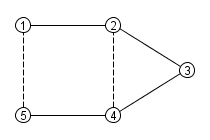
\includegraphics[width=3cm]{grafos_yed/g_34.jpg}
    \caption{Grafo $G_1$ de Exemplo para estudo de Busca em Profundidade.}
    \label{fig:g_34}
\end{figure}

A busca em profundidade aplicada ao algoritmo passando bp($G_1$,1), retorna a Tabela \ref{tab:t_1}:

\begin{table}[!htb]
    \small{
    \centering
	\begin{tabular}{|l|l|l|l|}
	    \hline
	    \multicolumn{1}{|c|}{\#} & \multicolumn{1}{c|}{chega} & \multicolumn{1}{c|}{sai} & \multicolumn{1}{c|}{pai} \\
	    \hline
	    \multicolumn{1}{|c|}{1} & \multicolumn{1}{c|}{1} & \multicolumn{1}{c|}{10} & \multicolumn{1}{c|}{-} \\
	    \hline
	    \multicolumn{1}{|c|}{2} & \multicolumn{1}{c|}{2} & \multicolumn{1}{c|}{9} & \multicolumn{1}{c|}{1} \\
	    \hline
	    \multicolumn{1}{|c|}{3} & \multicolumn{1}{c|}{3} & \multicolumn{1}{c|}{8} & \multicolumn{1}{c|}{2} \\
	    \hline
	    \multicolumn{1}{|c|}{4} & \multicolumn{1}{c|}{4} & \multicolumn{1}{c|}{7} & \multicolumn{1}{c|}{3} \\
	    \hline
	    \multicolumn{1}{|c|}{5} & \multicolumn{1}{c|}{5} & \multicolumn{1}{c|}{6} & \multicolumn{1}{c|}{4} \\
	    \hline
	\end{tabular}
    \caption{Tabela de Chega, Sai e Pai para a execu��o do algoritmo bp($G_1$,1).}
    \label{tab:t_1}
    }
\end{table}

As arestas $\{1,5\}$ e $\{2,4\}$ n�o s�o visitadas de forma expl�cita pelo algoritmo, ent�o essas arestas s�o chamadas de \textbf{arestas de retorno}, pois relacionam um v�rtice com um ancestral que n�o � o seu pai.

A Figura \ref{fig:g_35} mostra uma outra representa��o do grafo levando em considera��o as informa��es temporais.

\begin{figure}[!htb]
    \centering
    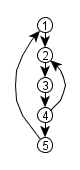
\includegraphics[width=1.2cm]{grafos_yed/g_35.jpg}
    \caption{Grafo $G_1$ Ordenado Temporalmente}
    \label{fig:g_35}
\end{figure}

Uma forma de conseguir atingir as arestas de retorno � a inser��o de um "SEN�O"{} entre as linhas 13 e 14 do C�digo \ref{alg:buscapro}.

As arestas que formam liga��es diretas com seus ancestrais s�o chamadas de arestas de �rvore. Por exemplo a aresta $\{1,2\}$.

\paragraph*{Exemplo 9:}

Seja um grafo $G_2$ representado pela Figura \ref{fig:g_36}

\begin{figure}[!htb]
    \centering
    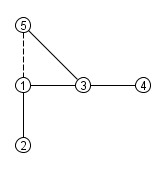
\includegraphics[width=2.5cm]{grafos_yed/g_36.jpg}
    \caption{Grafo $G_2$ de Exemplo para estudo de Busca em Profundidade.}
    \label{fig:g_36}
\end{figure}

\begin{table}[!htb]
    \centering
	\begin{tabular}{|l|l|l|l|}
	    \hline
	    \multicolumn{1}{|c|}{\#} & \multicolumn{1}{c|}{chega} & \multicolumn{1}{c|}{sai} & \multicolumn{1}{c|}{pai} \\
	    \hline
	    \multicolumn{1}{|c|}{1} & \multicolumn{1}{c|}{1} & \multicolumn{1}{c|}{10} & \multicolumn{1}{c|}{-} \\
	    \hline
	    \multicolumn{1}{|c|}{2} & \multicolumn{1}{c|}{2} & \multicolumn{1}{c|}{3} & \multicolumn{1}{c|}{1} \\
	    \hline
	    \multicolumn{1}{|c|}{3} & \multicolumn{1}{c|}{4} & \multicolumn{1}{c|}{9} & \multicolumn{1}{c|}{1} \\
	    \hline
	    \multicolumn{1}{|c|}{4} & \multicolumn{1}{c|}{5} & \multicolumn{1}{c|}{6} & \multicolumn{1}{c|}{3} \\
	    \hline
	    \multicolumn{1}{|c|}{5} & \multicolumn{1}{c|}{7} & \multicolumn{1}{c|}{8} & \multicolumn{1}{c|}{3} \\
	    \hline
	\end{tabular}
    \caption{Tabela de Chega, Sai e Pai para a execu��o do algoritmo bp($G_2$,1).}
    \label{tab:t_2}
\end{table}

A Figura \ref{fig:g_37} mostra uma outra representa��o do grafo levando em considera��o as informa��es temporais.

\begin{figure}[!htb]
    \centering
    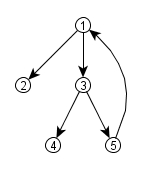
\includegraphics[width=2.2cm]{grafos_yed/g_37.jpg}
    \caption{Grafo $G_1$ Ordenado Temporalmente}
    \label{fig:g_37}
\end{figure}

A aresta $\{1,5\}$ s�o \textbf{arestas de retorno}, pois relaciona um v�rtice com um ancestral que n�o � o seu pai.

\subsection{Busca em Largura}

Para implementar a busca em largura basta trocar a escolha de um v�rtice no algoritmo base (C�digo \ref{alg:busca}) por uma fila.

A busca em largura acontece em camadas (n�veis) no grafo.

\paragraph*{Exemplo 10:} A Figura \ref{fig:g_38} mostra o mesmo grafo da busca em profundidade, entretanto a constru��o da �rvore de busca � dada de forma diferente.

\begin{figure}[!htb]
    \centering
    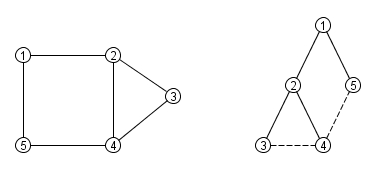
\includegraphics[width=5.5cm]{grafos_yed/g_38.jpg}
    \caption{Exemplo de Busca em Largura.}
    \label{fig:g_38}
\end{figure}

As arestas pontilhadas s�o chamadas de \textbf{arestas de cruzamento}, e as demais arestas s�o chamadas de \textbf{arestas de �rvore}.

\paragraph*{Observa��es:}

\begin{itemize}
    \item ao entrar na fila, um v�rtice tem o n�vel no m�ximo 1 a mais que o primeiro da fila;
    \item o n�vel dos v�rtices da fila � crescente.
\end{itemize}

\paragraph*{Conclus�o:}

\begin{itemize}
    \item os v�rtices da fila s�o de no m�ximo 2 n�veis;
    \item qualquer aresta do primeiro da fila para qualquer v�rtice na fila, liga v�rtices do mesmo n�vel ou 1 n�vel abaixo.
\end{itemize}

\paragraph*{Teorema:} Em uma busca em largura o n�vel em que se encontra um v�rtice � a dist�ncia para o v�rtice inicial?

\subsection{Algoritmos para Identificar Aresta de �vore ou de N�o-�rvore}

Os algoritmos que identificam as arestas de �rvore e de n�o �rvore a partir de um grafo e um v�rtice inicial, est�o dispostas nos Algoritmos \ref{alg:4} e \ref{alg:5}, que representam uma busca em largura e em profundidade respectivamente.

%    \begin{table*}
%        \texttt{\lstinputlisting[language=C, label=alg:aresta_lar,
%        caption={Identificar arestas para busca em largura.}]{cods/alg_aresta_lar.txt}}
%    \end{table*}
%
%    \begin{table*}
%        \texttt{\lstinputlisting[language=C, label=alg:aresta_pro,
%        caption={Identificar arestas para busca em profundidade.}]{cods/alg_aresta_pro.txt}}
%    \end{table*}

\begin{algorithm*}
    \small{
    \SetAlgoNoEnd
    $bfs(G,u)$\;
    \Inicio{
	$lista\_arestas\_visitadas[] \leftarrow \emptyset$\;
	$lista\_vertices\_visitados[] \leftarrow \emptyset$\;
	$lista\_arestas\_arvore[] \leftarrow \emptyset$\;
	$lista\_arestas\_nao\_arvore[] \leftarrow \emptyset$\;
	$lista\_auxiliar[] \leftarrow \emptyset$\;
	$lista\_vizinhos[] \leftarrow \emptyset$\;
	    adicione $v$ em lista\_vertices\_visitados\;
	    adicione $v$ em lista\_auxiliar\;
	\Enqto{lista\_auxiliar $\neq \emptyset$}{
	    $u$ = �ltimo elemento da lista\_auxiliar\;
	    remove o �ltimo elemento da lista\_auxiliar\;
	    lista\_vizinhos $\leftarrow n_g(u)$\;
	    \Enqto{lista\_vizinhos $\neq \emptyset$}{
		$w \leftarrow n_g(u)$\;
		\Se{na lista\_arestas\_visitadas $\not\in \{u,v\}$}{
		    adicione ${u,w}$ em lista\_arestas\_visistadas\;
		    \eSe{na lista\_vertices\_visitados $\not\in w$}{
			adicione $w$ na lista\_auxiliar\;
			adicione $w$ na lista\_vertices\_visitados\;
			adicione $\{u,w\}$ lista\_arestas\_nao\_arvore\;
		    }{
			adicione $\{u,w\}$ lista\_arestas\_arvore\;
		    }
		}
	    }
	}
    }
    \caption{Identificar arestas para busca em largura}
    \label{alg:4}
    }
\end{algorithm*}

\begin{algorithm*}
    \small{
    \SetAlgoNoEnd
    $dfs(G,u)$\;
    \Inicio{
	$lista\_arestas\_visitadas[] \leftarrow \emptyset$\;
	$lista\_vertices\_visitados[] \leftarrow \emptyset$\;
	$lista\_arestas\_arvore[] \leftarrow \emptyset$\;
	$lista\_arestas\_nao\_arvore[] \leftarrow \emptyset$\;
	$lista\_auxiliar[] \leftarrow \emptyset$\;
	$lista\_vizinhos[] \leftarrow \emptyset$\;
	\Enqto{lista\_auxiliar $\neq \emptyset$}{
	    $w$ � o v�rtice atual\;
	    $a$ � a aresta $\{v,w\}$\;
	    \Se{na lista\_arestas\_visitadas $\not\in a$}{
		adicione $a$ na lista\_arestas\_visitadas\;
		\eSe{na lista\_vertices\_visitados $\not\in w$}{
		    adicione $w$ na lista\_vertices\_visitados\;
		    adicione $a$ lista\_arestas\_arvore\;
		}{
		    adicione $a$ lista\_arestas\_nao\_arvore\;
		}
	    }
	}
    }
    \caption{Identificar arestas para busca em profundidade}
    \label{alg:5}
    }
\end{algorithm*}

\subsection{Aplica��es}

Dependendo do algoritmo que v� percorrer o grafo, os dois tipos de busca s�o eficientes e t�m o mesmo custo computacional, entretanto algumas particularidades de cada busca pode ser favor�vel para:

\begin{itemize}
    \item encontrar ciclos: utiliza-se busca em profundidade;
    \item caminho m�nimo: utiliza-se busca em largura.
\end{itemize}


    %%%%%%%%%%%%%%%%%%%%%%%
% C A P � T U L O   6 %
%%%%%%%%%%%%%%%%%%%%%%%

\chapter{Conexidade}

A conexidade diz respeito a qu�o \emph{conexo} � um grafo.

Um \textbf{grafo conexo} ou simplesmente \textbf{conexo} ou ainda \textbf{1-conexo} � um grafo que n�o cont�m partes separadas, ou formalmente: $G$ � conexo se � n�o vazio e quaisquer $2$ v�rtices de $G$ s�o extremos de um caminho em $G$.

Um grafo vazio por defini��o n�o � conexo, e um grafo de 1 v�rtice apenas, por defini��o � conexo.

\section{Componente Conexa}

Uma componente conexa � um subgrafo maximal conexo de $G$. Um subgrafo � maximal se n�o existe outro subgrafo maior que ele que tenha a mesma propriedade (no caso conexidade).

Uma defini��o formal para maximal �:

$X$ � maximal em uma propriedade $P$, se $X$ tem a propriedade $P$ e n�o pertence a $Y$ tal que $X \subset Y$ e $Y$ � $P$.

Para ilustrar o conceito de componente conexa vamos utilizar o grafo $G$ da Figura \ref{fig:g_39}.

\begin{figure}[!htb]
    \centering
    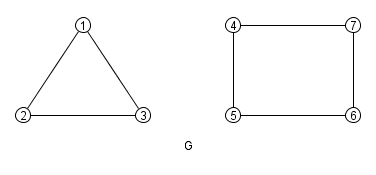
\includegraphics[width=6cm]{grafos_yed/g_39.jpg}
    \caption{Exemplo de componente conexa.}
    \label{fig:g_39}
\end{figure}

A componente conexa do grafo $G$ � dada pela indu��o $G[S] \therefore S = \{4,5,6,7\}$. Pois essa � a maior componente conexa poss�vel no grafo $G$. Se peg�ssemos um fragmento $S' = \{4,5\}$ poder�amos dizer que $G[S']$ � conexo entretanto n�o � uma componente conexa pois existe uma outra indu��o que tamb�m � conexa e maior que ela. Por esse motivo o formato triangular n�o pode ser considerado componente conexa, pois existe um quadrado que possui mais v�rtices que o tri�ngulo.

\section{Rela��o Bin�ria}

Seja $\sim_G$ a rela��o bin�ria entre dois v�rtices $u$ e $v$ definida como $u \sim_G v$ se e somente se:

\begin{itemize}
    \item existe um caminho em $G$ com extremos $u$ e $v$.
\end{itemize}

A rela��o $\sim_G$ � \emph{reflexiva}, \emph{sim�trica} e \emph{transitiva} o que define uma rela��o de equival�ncia.

\subsection{Fecho Transitivo}

O \textbf{fecho transitivo direto} de um v�rtice $v$ � o conjunto de todos os v�rtices que podem ser alcans�veis por algum caminho iniciando em $v$.

Seja o grafo $G$ da Figura \ref{fig:g_40}, ent�o:

\begin{figure}[!htb]
    \centering
    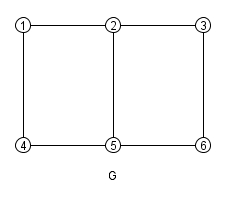
\includegraphics[width=3.5cm]{grafos_yed/g_40.jpg}
    \caption{Exemplo fecho transitivo.}
    \label{fig:g_40}
\end{figure}

\begin{itemize}
    \item O \textbf{fecho transitivo} do v�rtice $5$ do grafo $G$, por exemplo, � o conjunto: $\{1, 2, 3, 4, 5, 6\}$. Note que o pr�prio v�rtice faz parte do fecho transitivo j� que ele � alcan��vel partindo-se dele mesmo.
\end{itemize}

\section{Defini��es}

\begin{enumerate}
    \item Se $G$ � um grafo e $e$ � uma aresta de $G$, ent�o defina $G \smallsetminus e = (V(G), E(G) \smallsetminus \{e\})$.

    \item Se $G$ � um grafo e $v$ � um v�rtice de $G$, ent�o defina $G \smallsetminus v = (V(G) \smallsetminus \{v\}, E(G) \smallsetminus E_g(v))$.
\end{enumerate}

\section{Teorema do Ciclo}

Se $G = (V, E)$ � conexo ent�o $G \smallsetminus e$ � conexo para toda aresta $e$ que faz parte de um ciclo.

Para provar o teorema vamos ilustrar o teorema com o grafo $G$ da Figura \ref{fig:g_41}

\begin{figure}[!htb]
    \centering
    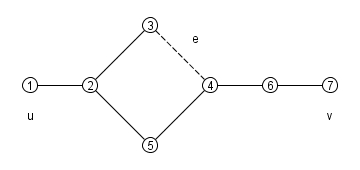
\includegraphics[width=6cm]{grafos_yed/g_41.jpg}
    \caption{Teorema: grafo conexo remo��o de aresta em ciclos.}
    \label{fig:g_41}
\end{figure}

� f�cil perceber que se removermos qualquer uma das arestas que est� no ciclo formado pelos v�rtices $\{2,3,4,5\}$ ainda poderemos obter um outro caminho de $u$ a $v$.

\paragraph*{Prova:} $u$ e $v \in V(G)$. Em $G$ existe um caminho de $u$ a $v$, esse caminho � dado por $C = (u = u_1, u_2, \ldots, u_k = v)$.

Podemos deduzir duas situa��es:

\begin{enumerate}
    \item Se $e$ n�o faz parte de $C$ ent�o $C$ tamb�m � caminho de $u$ a $v$ em $G \smallsetminus e$. Ou seja, se a aresta retirada n�o faz parte do meu caminho, n�o ter� influ�ncia nesse caminho.

    \item Se $e$ faz parte de $C$, ent�o:

    \begin{itemize}
	\item Define-se $e = \{x,y\}$;
	\item Defini-se $C = (u = u_1, u_2, \ldots, u_i = x, u_{i+1} = y, \ldots, u_k = v)$;
	\item Seja $C_1 = (u = u_1, u_2, \ldots, u_i)$;
	\item Seja $C_2 = (u_{i+1}, u_{i+2}, \ldots, u_k = v)$;
    \end{itemize}
\end{enumerate}

Como $e$ est� em um ciclo $L = (x, w_1, w_2, \ldots, w_n = y, x)$, ent�o existe um caminho $P$ de $x$ a $y$ que n�o cont�m a aresta removida.

Seja $T = (u = u_1, u_2, \ldots, u_i = x, w_1, \ldots, w_n = y, u_{i+2}, \ldots, w_k = v)$ um passeio formado por $T = (C_1 + P + C_2)$.

Ent�o existe um caminho entre dois v�rtices $u$ e $v$ em um passeio que contenha os v�rtices $u$ e $v$.

Defini-se $C'$ o caminho que � a simplifica��o de $T$, ent�o temos $C'$ um caminho de $u$ a $v$ em $G \smallsetminus e$.

\section{Articula��o}

Um v�rtice $v$ de um grafo conexo $G$ � uma \textbf{articula��o} (ou v�rtice de corte) se $G \smallsetminus v$ � n�o conexo.

O grafo $G$ da Figura \ref{fig:g_42} ilustra um v�rtice de articula��o:

  \begin{figure}[!htb]
    \centering
    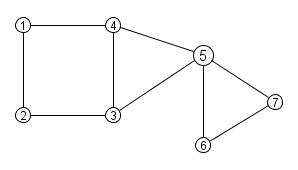
\includegraphics[width=5cm]{grafos_yed/g_42.jpg}
    \caption{V�rtice de articula��o.}
    \label{fig:g_42}
\end{figure}

O v�rtice $5$ � um v�rtice de articula��o, pois se o v�rtice $5$ for tirado do grafo o resultado ser� um grafo n�o conexo.

\section{Conexidade}

A \textbf{conexidade}, � o n�mero de v�rtices necess�rios para desconectar um grafo. O grafo da Figura \ref{fig:g_42} � 1-conexo, pois se removermos apenas um v�rtice (no caso o v�rtice 5) desconectamos o grafo.

Se $U \subseteq V(G)$ ent�o $G \smallsetminus U = G[V(G) \smallsetminus U]$.

Para todo $K \in \mathbb{N}$ dizemos que $G$ � K-conexo:

\begin{itemize}
    \item Se $|V(G)| [\geqslant, >] K$;
    \item Para todo $U \subset V(G)$, se $|U| < K$ ent�o $G \smallsetminus U$ � conexo;
\end{itemize}

A conexidade de um grafo $G$ � um n�mero $K(G)$ tal que $K(G) = \mbox{max}\{K \in \mathbb{N} \therefore G \mbox{ � conexo}\}$.

\paragraph*{Observa��o:} Pode-se definir tamb�m os mesmos conceitos de conexidade para arestas.

\section{Grafos Eulerianos}

Um grafo \emph{euleriano} � um grafo que pode ser desenhado sem retirar o l�pis do papel, dessa forma, uma aresta nunca ser� repetida.

\paragraph*{Defini��o Formal:} Um grafo $G$ � euleriano se em $G$ existe um passeio fechado (come�a e termina no mesmo lugar) sem repeti��es de arestas (trilha fechada) que passa por todas as arestas de $G$ e � conexo.

Uma \emph{trilha fechada} � um ciclo (circuito).

O grafo da Figura \ref{fig:g_43} � um grafo euleriano.

  \begin{figure}[!htb]
    \centering
    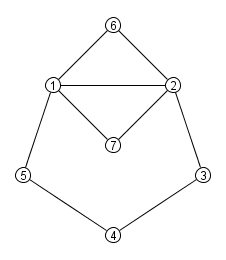
\includegraphics[width=4.5cm]{grafos_yed/g_43.jpg}
    \caption{Exemplo de Grafo Euleriano.}
    \label{fig:g_43}
\end{figure}

\subsection{Teorema de Euler}

Um grafo $G$ � \emph{euleriano} se e somente se $G$ � conexo e todo v�rtice tem grau par:

\paragraph*{Prova:} Ser euleriano implica em ser conexo e ter grau par ($\rightarrow$).

Se $G$ � euleriano, logo ele tamb�m � conexo.

Podemos assumir que existe uma trilha fechada que passa por todas a arestas de $G$.

Seja $v$ um v�rtice de $G$.

Se $v$ aparece na trilha $k$ vezes, ent�o o grau de $v$ � $2k$. Pois existe arestas que chegam e arestas que saem de $v$.

$G$ � conexo e todos os v�rtices t�m grau par ($\leftarrow$).

Seja $T = (v_0, v_1, v_2, \ldots, v_l)$ uma trilha com o maior n�mero poss�vel de arestas em $G$. $T$ passa por todas as arestas com extremos $v_0$ e $v_1$.

Se $v_0 \neq v_1$ o grau de $v_0$ deveria ser �mpar.

Como $v_0$ deve ter grau par, ent�o $v_0$ deve ser igual a $v_l$.

Logo, $T$ � fechado.

Suponha que existe uma aresta $e$ que n�o est� em $T$.

Pode-se assumir que $e = \{v_i,x\}$, j� que $G$ � conexo.

Pode-se re-escrever $T$ para que $v_i$ seja o primeiro v�rtice, portanto a trilha $T = (x, v_i, v_{i+1}, \ldots, v_l = v_0, v_1, v_2, \ldots, v_k)$ tem uma aresta a mais que $T$.

Logo, n�o existe aresta fora de $T$.

Logo, $T$ � fechada e passa por todas as arestas.

Portanto $G$ � euleriano.

\section{Grafos Hamiltorianos}

$G$ � \emph{hamiltoriano} se em $G$ existe um ciclo (circuito) que passa por todos os v�rtices.

\subsection{Teorema de Dirac}

Para todo grafo $G$ com 3 ou mais v�rtices se $\delta(G) \geqslant \frac{n}{2}$ ent�o $G$ � hamiltoriano.

\paragraph*{Prova:} Seja $P = (v_0, v_1, \ldots, v_l)$ o maior caminho em $G$ e defina os conjuntos:

\begin{itemize}
    \item $A = \{v_i em P \therefore \{v_0, v_{i+1} \in E(G)\}$
    \item $B = \{v_j em P \therefore \{v_l, v_j \in E(G)\}$
\end{itemize}

$A$ e $B$ s�o subconjuntos de $\{v_0,v_i,\ldots,v_{l-1}\}$.

$|A| \geqslant \frac{n}{2}$ e $|B| \geqslant \frac{n}{2}$.

$A \cap B \neq \emptyset$.

Seja $P = \{v_0, \ldots, v_k, v_{k+1}, \ldots, v_l\}$ se retirarmos a aresta $\{v_k, v_{k+1}\}$ e inserirmos uma equivalente $u$, ent�o podemos re-escrever $P$, e assim ele n�o � m�ximo.

\paragraph*{Observa��o:} O problema do caixeiro viajante tem uma rela��o com os grafos hamiltorianos, pois passar por todas as cidades sem repeti��es, � tamb�m uma caracter�stica da propriedade estudada.

\section{Caminhos M�nimos em Grafos com Pesos nas Arestas}

Nessa se��o iremos estudar grafos que possuem pesos em suas arestas, ou seja, o fator que deixa um caminho maior ou menos n�o est� apenas na contagem de arestas, mas no somat�rios dos pesos de todas as arestas que fazem parte desse caminho.

Uma \emph{defini��o formal} diz que um grafo com pesos nas arestas � uma terna $(V,E,\omega)$ onde $V$ e $E$ s�o os usuais conjuntos de v�rtices e arestas, respectivamente, e $\omega: E(G) \rightarrow \mathbb{R}^+$ � uma fun��o que atribui peso a cada aresta de $E(G)$.

Por exemplo o grafo $G$ da Figura \ref{fig:g_44}.

  \begin{figure}[!htb]
    \centering
    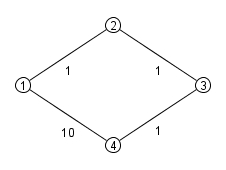
\includegraphics[width=4.5cm]{grafos_yed/g_44.jpg}
    \caption{Exemplo de Grafo com Pesos nas Arestas.}
    \label{fig:g_44}
\end{figure}

O \emph{comprimento de um caminho} $C = (x_0, x_1, \ldots, x_k)$ em $(V,E,\omega)$ � a soma dos pesos (comprimentos) das arestas do caminho, ou seja:

$$ \mbox{custo}(C) = \sum_{i=0}^{k-1} p(\{x_i, x_{i+1}\}) $$

E a \emph{dist�ncia} entre dois v�rtices $u$ e $v$ � dada por:

$$ \mbox{dist}(u,v) = min\{ \mbox{custo}(C) \} $$

Sendo que  $C$ � um caminho com extremos em $u$ e $v$.

Se n�o existe um caminho de $u$ a $v$ ent�o assume-se que $ \mbox{dist}(u,v) = \infty $.

\subsection{Algoritmo de Dijkstra para Caminhos M�nimos}

Suponha que � dado um grafo com pesos nas arestas do tipo $G = (V,E, \omega)$ e um v�rtice $s \in V(G)$. Pede-se para determinar a dist�ncia de $s$ a todos os v�rtices de $G$, ou formalmente: $\mbox{dist}(u,v) \therefore v \in V(G)$.

As estruturas de dados que ser�o utilizadas s�o:

\begin{itemize}
    \item $P[v]$: Predecessor de $v$ em um caminho \emph{candidato} a ser m�nimo de $s$ a $v$;
    \item $D[v]$: Custo do caminho \emph{candidato} a ser m�nimo;
    \item $S$: Conjunto dos v�rtices para os quais $D[v]$ � equivalente a $\mbox{dist}(s,v)$.
\end{itemize}

Inicialmente, as estruturas est�o:

\begin{itemize}
    \item $P[v] = \lambda$ para todo $v \in V(G)$;
    \item $D[v] = \emptyset$ para todo $v \in V(G) \smallsetminus \{s\}$;
    \item $S    = \emptyset$;
\end{itemize}

Uma etapa importante chamada de relaxa��o � definida pelo algoritmo do Algoritmo \ref{alg:6}.

\begin{algorithm}
    \SetAlgoNoEnd
    $Relaxacao(u,t)$\;
    \Inicio{
	\Se{ $d[t] > d[u] + \omega(\{u,t\})$ }{
	    $dt[t] \leftarrow d[u] + \omega(\{u,t\})$\;
	}
    }
    \caption{Relaxa��o($u,t$)}
    \label{alg:6}
\end{algorithm}

Essa fun��o de \emph{Relaxa��o($u,v$)} compara se a dist�ncia de determinado v�rtice a outro � menor, se for atribui a ele a nova dist�ncia.

O algoritmo completo de Dijkstra est� representado pelo Algoritmo \ref{alg:7}.

O algoritmo come�a com um conjunto $S$ vazio. A cada itera��o do algoritmo, busca-se em uma lista de prioridades o v�rtice que possui a menor dist�ncia. Por esse motivo o primeiro passo � adicionar $u$ ao conjunto $S$ (que tem a dist�ncia inicial $0$, pois $\mbox{dist}(u,u) = 0$). A dist�ncia para qualquer outro $v \in V(G) = \infty$. Um conjunto $\overline{S}$ cont�m os demais v�rtices de $V(G)$. O pr�ximo passo � listar os vizinhos $v$ de $u$ e executar a subrotina de \emph{relaxa��o} para garantir que se houver um caminho mais curto, esse ser� o novo $D[v]$, permitindo assim que em uma pr�xima itera��o esse seja o menor na lista de prioridades e seja escolhido.

\begin{algorithm}
    \small{
    \SetAlgoNoEnd
    \Inicio{
	$D[u] \leftarrow \infty$\;
	$P[u] \leftarrow \lambda$\;
	$D[s] \leftarrow \emptyset$\;
	$S \leftarrow \{\}$\;
	\Enqto{existir $u \in \overline{S}$ tal que $D[u] \neq \infty$}{
	    seja $u$ tal que $d[u] = \mbox{min}\{d[v] \therefore v \in \overline{S}\}$\;
	    \ParaCada{$t \in N_G(u)$}{
		Relaxa��o($u,t$)\;
	    }
	    $S \leftarrow S \cup \{u\}$\;
	}
    }
    \caption{Dijkstra($G,u$)}
    \label{alg:7}
    }
\end{algorithm}

O custo do algoritmo de Dijkstra para obten��o do caminho m�nimo � $\Theta((n+m)\log_n)$.

\subsection{Algoritmo de Floyd-Warshall para caminhos m�nimos}

Seja $G = (V, E, \omega)$ um grafo com pesos nas arestas. Apresenta-se um algoritmo
para resolver o seguinte problema: dado $G = (V, E, \omega)$ computar $dist_G(i, j)$ para todos $i, j \in V$.

Uma alternativa para realizar essa tarefa � utilizar $n$ vezes com $n = |V(G)|$ o algoritmo de Dijkstra.

Seja a representa��o de $G$ dada pela matriz:

$$
a _{i,j} =   \left\{ \begin{array}{cll}
			0 & \mbox{se} & i = j \\
			\omega(\{i,j\}) & \mbox{se} & \{i,j\} \in E(G) \\
			\infty & & \mbox{caso contr�rio.}
		    \end{array}\right.
$$

\paragraph*{Defini��es:}

\begin{enumerate}
    \item Para todo $k \in \{0,1,\ldots,|V|\}$ denotamos por $[k]$ o subconjunto $\{1, 2, \ldots, k\} \subseteq V$, com $[0] = \emptyset$;

    \item Dizemos que o caminho $P = (i, v_0, \ldots, v_t, j)$ � um [k]-caminho se o seus v�rtices internos $\{v_0, \ldots, v_t\}$ pertencem a $[k]$;

    \item Uma [k]-dist�ncia entre $i$ e $j$ � o comprimento do menor [k]-caminho com extremos em $i$ e $j$. Denotada por $dist_k(i,j)$, com $dist_0(i,j) = a_{i,j}$.
\end{enumerate}

\paragraph*{Exemplo 11:} Seja o grafo $G$ representado pela Figura \ref{fig:g_45}.

  \begin{figure}[!htb]
    \centering
    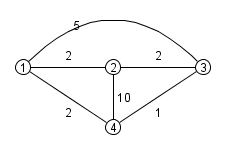
\includegraphics[width=4cm]{grafos_yed/g_45.jpg}
    \caption{Exemplo dos conceitos para algoritmo de Floyd-Warshall.}
    \label{fig:g_45}
\end{figure}

Para entender melhor vamos analisar o grafo $G$.

\begin{itemize}
    \item o �nico [0]-caminho com extremos $3$ e $4$ � $\{3,4\}$;

    \item os [1]-caminhos com extremos $3$ e $4$ s�o $\{3,4\}$ e $\{3,1,4\}$;

    \item os [2]-caminhos com extremos $3$ e $4$ s�o $\{3,4\}$ e $\{3,1,4\}$;

    \item os [3]-caminhos com extremos $3$ e $4$ s�o $\{3,2,4\}, \{3,1,4\}$;

    \item os [4] caminhos com extremos $3$ e $4$ s�o $\{3,1,2,4\}, \\ \{3,2,1,4\}$.
\end{itemize}

No grafo $G$ temos $dist_0(3,4) = 5$, $dist_1(3,4) = 4$ e $dist_2(3,4) = dist_3(3,4) = dist_4(3,4) = 3$. E ainda, $dist_0(1,2) = dist_1(1,2) = dist_2(1,2) = 10$, $dist_3(1,2) = 4$ e $dist_4(1,2) = 3$.

\subsection{Algoritmo de Floyd-Warshall}

A id�ia principal do algoritmo � que podemos obter $dist_{k+1}$ a partir de $dist_k$ da seguinte maneira: por defini��o, a $dist[k+1]-dist$ � o comprimento do menor $[k+1]$-caminho e a $[k]$-dist�ncia � o comprimento do menor $[k]$-caminho; logo, a diferen�a entre esses caminhos � que no primeiro, os $[k+1]$-caminhos, � poss�vel que o v�rtice $k+1$ seja o v�rtice interno e no segundo n�o, pois $[k + 1] = [k] \cup \{k + 1\}$.

Assim temos:

$$ dist_{k+1}(i,j) = min\{dist_k(i,j), (dist_k(i,k+1) + dist_k(k+1,j))\} $$

Escrevendo o algoritmo, obtemos o Algoritmo \ref{alg:8}.

\begin{algorithm}
    \small{
    \SetAlgoNoEnd
    \Entrada{um grafo $G$ com peso $\omega$ nas arestas.}
    \Saida{$dist_G{i,j}$ para todos $(i,j) \in V(G)$.}
    \Inicio{
	\ParaCada{$(i,j) \in V(G)^2$}{
	    $dist_0(i,j) \leftarrow a_{i,j}$\;
	    \ParaCada{$k$ de 1 at� $|V(G)|$}{
		\ParaCada{$(i,j) \in V(G)^2$}{
		    $dist_k(i,j) \leftarrow min\{dist_{k-1}(i,j), (dist_{k-1}(i,k) + dist_{k-1}(k,j))\}$\;
		}
	    }
	}
    }
    \caption{Floyd-Warshall($G$)}
    \label{alg:8}
    }
\end{algorithm}


    %%%%%%%%%%%%%%%%%%%%%%%
% C A P � T U L O   7 %
%%%%%%%%%%%%%%%%%%%%%%%

\chapter{�rvores}

As �rvores estudadas em grafos podem ser consideradas \textbf{�rvores gen�ricas}. Nesse tipo de �rvore pouco importa quem � o seu nodo raiz, pois a qualquer momento pode-se eleger um nodo e tornalo raiz. Esse recurso � dispon�vel pela estrutura com que o grafo est� disposo.

Uma �rvore � um grafo que possui apenas o n�mero suficiente de arestas para que esse grafo n�o seja desconexo, e ao mesmo tempo n�o contenha ciclos.

Para introduzir os conceitos de �rvores, vamos primeiro definir uma \textbf{floresta}.

\section{Floresta}

Uma \textbf{floresta} � um grafo cujas componentes conexas n�o cont�m circuito (ciclo).

\section{�rvores}

Defini-se como \textbf{�rvore}, os componentes conexos de uma floresta, ou seja, uma �rvore � um grafo conexo e sem circuitos.

\section{Folha}

Uma \textbf{folha} � um v�rtice de grau um na �rvore.

\paragraph*{Exemplo 12:} O Grafo $G$ da Figura \ref{fig:g_46}, � uma floresta, e cada uma de suas componentes conexas s�o �rvores. As folhas dessa floresta s�o: $2,3,8,7,5,10,13,12$.

\begin{figure}[!htb]
  \centering
  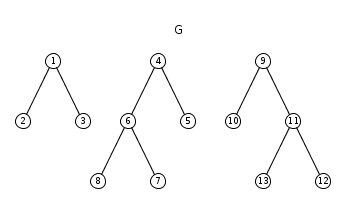
\includegraphics[width=6cm]{grafos_yed/g_46.jpg}
  \caption{Exemplo de Floresta e �rvores.}
  \label{fig:g_46}
\end{figure}

\section{�rvore Geradora}

Uma �rvore geradora de um grafo $G$ � um subgrafo gerador $T$ de $G$ tal que $T$ � gerador e � uma �rvore.

\subsection{Teorema ($n-1$)}

Provar que uma �rvore possui o n�mero de arestas igual ao n�mero de v�rtices menos um. Ou formalmente $|E(G) = |V(G)| - 1$. Defini-se $n = |V(G)|$.

\paragraph*{Prova:} Por defini��o uma �rvore $G$ possui as propriedades:

\begin{itemize}
  \item $G$ � ac�clico, o que implica em $|E(G)| \leqslant n - 1$
  \item $G$ � conexo, o que implica em $|E(G)| \geqslant n - 1$
\end{itemize}

Como $G$ possui as duas propriedades, logo:

\begin{eqnarray*}
  |E(G)| &\leqslant& n - 1 \\
  |E(G)| &\geqslant& n - 1 \\
  |E(G)| &=& n-1
\end{eqnarray*}

\subsection{Teorema da Folha}
\label{teo:grau1arv}

Toda �rvore com mais de um v�rtice tem pelo menos uma folha.

\paragraph*{Prova:} Seja uma �rvore $G$ e suponha que $\delta(G) \geqslant 2$.

Todo grafo $G$ cont�m um caminho de comprimento pelo menos $\delta(G)$ e se $\delta(G) \geqslant 2$ esse grafo tamb�m possui um ciclo de tamanho $\delta(G) + 1$.

Logo, $G$ cont�m ciclos e n�o � uma �rvore.

\subsubsection{Color�rio da Folha}

Todo grafo ac�clico com pelo menos uma aresta tem pelo menos um v�rtice de grau 1.

\paragraph*{Prova:} Seja $G$ um grafo ac�clico com pelo menos 1 aresta, tome uma componente conexa $H$ de $G$ que contenha pelo menos uma aresta.

$H$ � ac�clica, pois � subgrafo de $G$. $H$ cont�m pelo menos dois v�rtices, j� que possui arestas.

Logo, $H$ � uma �rvore e cont�m folhas.

\subsubsection{Lema da Folha}

Todo grafo conexo e com $m = n-1$ tal que $n > 1$, tem um v�rtice de grau 1. Sendo que $m$ � $|E(G)$ e $n$ � $|V(G)|$.

\paragraph*{Prova:} Seja $G$ um grafo conexo com $m = n-1$.

Sabe-se que $\displaystyle\sum_{v \in V(G)} d_G(v) = 2|E(G)|$. Logo podemos deduzir que: $\displaystyle\sum_{v \in V(G)} d_G(v) = 2n-2$.

\begin{eqnarray*}
  \sum_{v \in V(G)} d_G(v) = \sum_{v \in V(G)} (d_G(v) - \delta(G)) + n \delta(G) = 2n-2 \\
  \sum_{v \in V(G)} (d_G(v) - \delta(G)) = n(2 - \delta(G)) - 2 \\
  \sum_{v \in V(G)} (d_G(v) - \delta(G)) \geqslant 0, \mbox{ pois } d_G(v) \geqslant 0
\end{eqnarray*}

Logo, $n(2 - \delta(G)) - 2 > 0$. Para isso: $\delta(G) < 2$.

Ao mesmo tempo, como $G$ � conexo, temos que $\delta(G) \geqslant 1$, logo $\delta(G) = 1$.

\subsection{Teorema da Prova dos 3}

Seja $G$ um grafo com $n$ v�rtices e $m$ arestas, se $G$ tem duas das seguintes propriedades, ent�o tamb�m tem a terceira:

\begin{enumerate}
\item\label{t1} $m = n-1$;
\item\label{t2} $G$ � conexo;
\item\label{t3} $G$ � ac�clico.
\end{enumerate}

Provar que:

\begin{itemize}
  \item[I)] \ref{t1} e \ref{t2} $\rightarrow$ \ref{t3};

  \paragraph*{Base:} Seja o grafo $G$ trivial ($n=1$). Obviamente � ac�clico.

  \paragraph*{Hip�tese de Indu��o:} Suponha que todo grafo conexo com $n = k-1$ e $m = k-2$ seja ac�clico.

  \paragraph*{Passo:} Seja $G$ um grafo conexo com $n = k$. Tome uma folha $v \in V(G)$. Considere o grafo $G' = G \smallsetminus v$. Assim temos que:

  \begin{eqnarray*}
      |V(G')| &=& |V(G)| - 1 = k - 1 \\
      |E(G')| &=& |E(G)| - d_G(v) = k - 1 - 1 = k - 2
  \end{eqnarray*}

  Como chega-se a $k-1 = n$ e $k-2 = m$, descrito pela \textit{Hip�tese de Indu��o}, podemos afirmar que:

  $G$ � conexo e $d_G(v) = 1$ logo, $G'$ � conexo.

  Pela \textit{Hip�tese de Indu��o} $G'$ � ac�clico.

  Como $d_G(v) = G$, $G$ tamb�m � ac�clico.

  \item[II)] \ref{t1} e \ref{t3} $\rightarrow$ \ref{t2};

  \paragraph*{Base:} Seja o grafo $G$ trivial ($n=1$). Obviamente � conexo.

  \paragraph*{Hip�tese de Indu��o:} Suponha que todo grafo ac�clico com $n = k-1$ e $m = k-2$ seja conexo.

  \paragraph*{Passo:} Seja $G$ um grafo ac�clico com $n = k$. Tome uma folha $v \in V(G)$. Considere o grafo $G' = G \smallsetminus v$. Assim temos que:

  \begin{eqnarray*}
      |V(G')| &=& |V(G)| - 1 = k - 1 \\
      |E(G')| &=& |E(G)| - d_G(v) = k - 1 - 1 = k - 2
  \end{eqnarray*}

  Como chega-se a $k-1 = n$ e $k-2 = m$, descrito pela \textit{Hip�tese de Indu��o}, podemos afirmar que:

  $G$ � ac�clico logo, $G'$ � ac�clico.

  Pela \textit{Hip�tese de Indu��o} $G'$ � conexo.

  Logo, $G$ tamb�m � conexo.

  \item[III)] \ref{t2} e \ref{t3} $\rightarrow$ \ref{t1}.

  \paragraph*{Base:} Seja o grafo $G$ trivial ($n=1$). Obviamente $m = 0$ e $m = n - 1$.

  \paragraph*{Hip�tese de Indu��o:} Suponha que todo grafo ac�clico e conexo (�rvore) com $n = k-1$ tenha $m = k-2$.

  \paragraph*{Passo:} Seja $G$ uma �rvore com $n = k$. Tome uma folha $v \in V(G)$. Considere o grafo $G' = G \smallsetminus v$. Assim temos que:

  $G$ � conexo e $d_G(v) = 1$ $\rightarrow$ $G'$ � conexo;

  $G$ � ac�clico $\rightarrow$ $G'$ � ac�clico, pois a remo��o de um v�rtice nunca poder� tornar um grafo ac�clico.

  \begin{eqnarray*}
      |V(G')| &=& |V(G)| - 1 = k - 1 \\
      |E(G')| &=& \big[ |V(G) -1 \big] - 1 = k-2
  \end{eqnarray*}

  Como $G'$ � ac�clico e conexo, e a retirada de uma de suas folhas, comprova a \textit{Hip�tese de Indu��o} por:

  \begin{eqnarray*}
      n &=& |V(G)| - 1\\
      d_G(v) &=& 1\\
      |V(G')| &=& n = k - 1\\
      |E(G')| &=& n - d_G(v) = k-2\\
      m &=& n-1
  \end{eqnarray*}

  A demonstra��o $n = k-1$ prova a primeira \textit{Hip�tese de Indu��o}. e a demonstra��o $n - d_G(v) = k-2$ prova a segunda \textit{Hip�tese de Indu��o}.

  Logo, pode-se inferir $m = n-1$

\end{itemize}

\subsection{Teorema da Prova dos 4}

Antes de enunciar e provar uma caracteriza��o define-se a opera��o:

$G$ � um grafo e $x,y \in V(G)$. Denota-se:

$$ G + xy = (V(G), E(G)\cup\{x,y\})$$

As seguintes afirma��es s�o equivalentes para todo grafo $G = (V,E)$:

\begin{itemize}
  \item[(1)] $G$ � �rvore;
  \item[(2)] para quaisquer $x,y \in V(G)$ existe um �nico caminho em $G$ com extremos $x$ e $y$;
  \item[(3)] $G$ � conexo minimal: $G$ � conexo e $G \smallsetminus e$ � desconexo, para qualquer $e \in E(G)$;
  \item[(4)] $G$ � ac�clico maximal: $G$ � ac�clico e $G + xy$ cont�m um circuito, para quaisquer $x,y \in V(G)$ n�o adjacentes. 
\end{itemize}

Para provar que essas afirma��es s�o equivalentes devemos mostrar que:

$$ (1) \rightarrow (2) \rightarrow (3) \rightarrow (4) \rightarrow (1) $$

\paragraph*{Provar que $(1) \rightarrow (2)$}

Como $G$ � conexo, existe um caminho 

$$P = (x = x_0, x_1, \ldots, x_n-1, x_n = y)$$

Suponha a exist�ncia de um outro caminho 

$$Q = (x = y_0, y_1, \ldots, y_m-1, y_m = y)$$

Pode ser que esses caminhos tenham seus v�rtices iniciais contidos em um mesmo caminho, por isso � necess�rio definir bem os �ndices para explicitar que pelo menos um ciclo ir� ser identificado.

Ent�o, sejam os �ndices:

\begin{eqnarray*}
  r &=& min(i: i \geqslant 0 \mbox{ e } x_{i+1} \neq y_{i+1}) \\
  s &=& min(j: i > p \mbox{ e } x_j = y_l \mbox{ para algum } l > p)
\end{eqnarray*}

O �ndice $r$ identifica o primeiro v�rtice do caminho $P$ que seja diferente no caminho $Q$.

O �ndice $s$ identifica o primeiro v�rtice maior que o v�rtice indexado pelo �ndice $r$, tal que exista um v�rtice $x_j$ do caminho $P$ igual a um v�rtice $y_l$ do caminho $Q$ tal que o indice l seja maior que o indice p definido.

Esses �ndices est�o bem definidos, como os caminhos s�o distintos, temos: $0 \leqslant r < min\{m,n\}$ e $r < s \leqslant n+1$.

Dessa forma conseguimos montar um circuito dado por:

$T = (x_r, x_{r+1}, \ldots, x_s = y_l, y_{l-1}, y_{l-2},y_r)$

Assim temos uma contradi��o, e podemos afirmar que o caminho com extremos $x,y$ � �nico.

\paragraph*{Demonstra��o:} Pode ser dada por:

Seja $V(G) = X \cup \overline{X} \therefore X \cap \overline{X} = \emptyset$.

Seja $C_1$ um caminho de um v�rtice $v$ a um v�rtice $a \subset X$.

Seja $C_2$ um caminho de um v�rtice $y$ a um v�rtice $b \subset \overline{X}$.

� poss�vel adicionar os sucessores de de $a$ e $b$ ao caminho $C_1$ e $C_2$ respectivamente, at� que entre $a_n$ e $b_n$ possua apenas um v�rtice $c$ que possui as arestas $\{a_n,c\},\{b_n,c\}$.

Dessa forma s� existe um caminho de $v$ a $a_n$ pois todos os sucessores de $a$ foram adicionados ao conjunto $X$. e tamb�m s� existe um caminho de $y$ a $b_n$ pelo mesmo motivo com $\overline{X}$.

Como o v�rtice $c$ � o �nico que liga $a_n$ e $b_n$, logo s� existe um caminho entre $v$ e $y$.

\paragraph*{Provar que $(2) \rightarrow (3)$}

Seja $G$ tal que $(2)$ vale, ent�o $G$ � conexo ent�o existe um caminho para qualquer par de v�rtices $x$ e $y$ tal que $x,y \in V(G)$.

Tome $\{x,y\} \in E(G)$ temos que

$C = (x = v_0, v_1, \ldots, v_{n-1}, v_n = y)$ � o �nico caminho entre $x$ e $y$.

Temos que ao remover uma aresta de um caminho �nico torna o grafo desconexo, ent�o:

$C \smallsetminus e$ � desconexo, para qualquer $e \in E(G)$.

Se existe um �nico caminho ligando $x$ a $y$, o grafo � conexo, logo podemos afirmar que $(2) \rightarrow (3)$.

\paragraph*{Provar que $(3) \rightarrow (4)$}

Suponha que $G$ seja c�clico. Ent�o � poss�vel retirar qualquer aresta pertencente a um ciclo de $G$ e $G \smallsetminus e \therefore e \in E(G)$ continua conexo.

Logo, $G$ � ac�clico, pois n�o � poss�vel retirar qualquer aresta pela defini��o $(3)$.

Sejam $x$ e $y$ n�o adjacentes em $G$, como $G$ � conexo, ent�o existe um caminho $C = (x = v_0, v_1, \ldots, v_{n-1}, v_n = y)$.

Considere o grafo $G' = G + \{x,y\}$. Logo, $C' = (x = v_0, v_1, \ldots, v_{n-1}, v_n = y, x)$. Ent�o $C'$ � um ciclo em $G'$.

Logo, $G$ � um grafo ac�clico maximal.

Como s� � poss�vel adicionar a aresta entre as extremidades do caminho achado, o grafo $G$ � ac�clico e maximal.

\paragraph*{Provar que $(4) \rightarrow (1)$}

Suponha que $G$ seja desconexo. $x$ e $y$ s�o dois v�rtices entre os quais n�o h� caminho em $G$.

Seja $G' = G + \{x,y\}$, temos que $G'$ � ac�clico, contrariando que $G$ pudesse ser maximal, logo, $G$ � conexo.

Sendo conexo, o grafo $G$ � uma �rvore.

\section{�rvores Geradoras de Custo M�nimo em Grafos com Pesos nas Aresta}

Defini-se como custo de um subgrafo $H$ de $G$ conexo e com peso nas arestas $G = (V,E,\omega)$, onde $\omega : E \rightarrow \mathbb{R}$:

$$
c(H) = \sum_{e \in E(H)} \omega(e)
$$

O problema a ser atacado � a resposta para a pergunta: Qual � o menor custo do subgrafo gerador conexo de $G$?

Ou formalmente, $S \subseteq E(G)$ que induz a uma �rvore geradora de $G$ tal que:

$$ 
c(G[S]) = min\{c(T): T \mbox{ � �rvore geradora de } G\}
$$

Uma �rvore geradora de $G$ de custo m�nimo tamb�m � chamada de \textbf{�rvore geradora m�nima} do grafo $G$.

Apresenta-se a seguir os algor�tmos de \textit{Jarn�k-Prim} e \textit{Kruskal} para resolver o problema de determinar a �rvore geradora m�nima.

Esses algoritmos s�o gulosos, que � uma t�cnica de projeto de algoritmos para resolver problemas de otimiza��o. os c�digos baseam-se na escolha que parece ser a melhor no momento (�timo local) e terminam com a solu��o �tima (�timo global).

\section{Algoritmo de Jarn�k-Prim para �rvore geradora m�nima}

Seja $X$ um conjunto de v�rtices tal que $X \subset V(G)$ e $X$ n�o � vazio. Temos ainda $\overline{X}$ que � o complemento de $X$.

\subsection{Teoremas de Prim}

\begin{enumerate}
  \item\label{teo:prim:1} Toda �rvore geradora possui pelo menos uma aresta de $E(X,\overline{X})$;
  \item\label{teo:prim:2} Uma �rvore geradore m�nima, possui uma das arestas de menor peso em $E(X,\overline{X})$.
\end{enumerate}

Com os teoremas \ref{teo:prim:1} e \ref{teo:prim:2} podemos estabelecer uma rela��o com o corte $E(X,\overline{X})$ e as arestas de menor peso da �rvore geradora m�nima.

O algor�tmo de \textit{Jarn�k-Prim} divide o grafo em dois conjuntos, os v�rtices que foram visistados $U$, e os que n�o foram visistados $\overline{U}$. E a cada itera��o adiciona para o conjunto $U$ o v�rtice que tinha a aresta de menor peso dentre todas as arestas do corte $E(U,\overline{U})$. Esse processo � repetido at� que $U = V(G)$. No final do processo $G[U]$ � uma �rvore geradora m�nima.

O Algor�tmo \ref{alg:9} descreve a estrat�gia de Jarn�k-Prim.

\begin{algorithm}
    \small{
    \SetAlgoNoEnd
    \Entrada{um grafo $G$ com peso $\omega$ nas arestas.}
    \Saida{arvore geradora de custo m�nimo.}
    \Inicio{
	escolha $v \in V(G)$\;
	$U \leftarrow \{v\}$\;
	$S \leftarrow \emptyset$\;
    
	\Enqto{$U \neq V(G)$}{
	  escolha $\{u,w\} \in E(U,\overline{U})$ de peso m�nimo no corte\;
	  insira $\{u,w\}$ em $S$\;
	  $v \leftarrow \{u,w\} \cap \overline{U}$\;
	  insira $v$ em $U$\;
	}
	devolva $(V,S)$
    }
    \caption{Jarn�k-Prim($G$)}
    \label{alg:9}
    }
\end{algorithm}

O principal gasto computacional est� relacionado a escolha das arestas de menor peso. Claramente � invi�vel que a cada procura para achar a aresta de menor peso, visite-se todas as arestas que incidem no v�rtice em quest�o.

Para melhorar essa implementa��o, prop�e-se o uso de uma fila de prioridades que armazena as arestas priorizando o seu peso. Recomenda-se a utiliza��o de uma estrutura \textit{Heap} para melhorar a efici�ncia do algoritmo.

Ent�o basta encontrar na lista de prioridades uma ocorr�ncia do v�rtice em quest�o, e sacar essa aresta.

O Algoritimo \ref{alg:10} � uma implementa��o da fila de prioridades baseado no Algoritimo \ref{alg:9}.

\begin{algorithm}
    \small{
    \SetAlgoNoEnd
    \Entrada{um grafo $G$ com peso $\omega$ nas arestas.}
    \Saida{arvore geradora de custo m�nimo.}
    \Inicio{
	escolha $v \in V(G)$\;
	$U \leftarrow \{v\}$\;
	$S \leftarrow \emptyset$\;
	$L \leftarrow$ lista de prioridades por pesos das arestas\;
    
	\Enqto{$U \neq V(G)$}{
	  $w \leftarrow$ o outro v�rtice da aresta $\{u,w\}$ que seja a primeira ocorr�ncia em $L$\;
	  insira $\{u,w\}$ em $S$\;
	  $v \leftarrow w$\;
	  insira $v$ em $U$\;
	}
	devolva $(V,S)$
    }
    \caption{Jarn�k-Prim($G$)}
    \label{alg:10}
    }
\end{algorithm}

\subsection{Avalia��o de Corretude}

\paragraph*{Teorema de Jarn�k-Prim:}\label{teo:prim} Para $k \in \mathbb{N}$, ap�s $k$ itera��es do "enquanto"{} do algoritmo de \textit{Jarn�k-Prim}, as arestas escolhidas induzem uma sub �rvore de uma �rvore geradora m�nima.

\paragraph*{Defini��es}

Para provar o teorema, vamos fazer algumas defini��es:

\begin{itemize}
  \item $S_0 = \emptyset$;
  \item $S_1 = \{v\}$;
  \item $A_0 = \emptyset$;
  \item $A_1 = \emptyset$.
\end{itemize}

Sendo que o conjunto $S$ � o conjunto de v�rtices visistados, e o conjunto $A$ � o conjunto de arestas que formar�o uma �rvore geradora m�nima.

A cada volta do algoritmo, escolhe-se uma aresta $e$ do corte com peso m�nimo.

Ent�o temos:

\begin{eqnarray*}
    e &=& \{u,w\} \in E(S_i, \overline{S_i}) \\
    u &\in& S_i \\
    w &\in& \overline{S_i} \\
    S_{i+1} &=& S_i \cup \{w\} \\
    A_{i+1} &=& A \cup \{\{u,w\}\}
\end{eqnarray*}

\subsubsection{Prova do Teorema de Jarn�k-Prim}

Podemos ent�o reescrever o Teorema \ref{teo:prim} da seguinte maneira: $(S_k, A_k)$ � uma sub�rvore de uma �rvore geradora m�nima.

Devemos provar que:

\begin{itemize}
  \item $(S_k, A_k)$ � uma �rvore;
  \item $(S_k, A_k) \subset T_{min}$;
\end{itemize}

Sendo que $T_{min}$ � uma �rvore geradora m�nima.

Para provar que $(S_k, A_k)$ � uma �rvore, temos que provar que a cada passo, cada v�rtice ou aresta adicionados em $S$ e $A$ ainda deixam a �rvore conexa e ac�clia.

\begin{itemize}
  \item \textit{Ac�clico}: Como $S$ s� possui aresta de menor peso entre seus elementos, ent�o os elementos de $S$ n�o mais mais de uma aresta para qualquer outro elemento de $S$. O que garante a n�o exist�ncia de ciclos.
  \item \textit{Conexo}: A conexidade � garantida pois, como $S$ come�a com um v�rtice (por defini��o conexo), e a cada inser��o em $S$ tem-se uma aresta que liga os elementos do corte $E(S,\overline{S})$, ent�o ao final da execu��o, a �rvore geradora m�nima permanecer� conexa.
\end{itemize}

Para provar que $(S_k, A_k) \subset T_{min}$.

Tomamos como \textbf{base} um grafo trivial.

Temos a seguinte \textbf{hip�tese}:

Para $0 \leqslant k \leqslant a$ ent�o $(S_k, A_k) \subseteq T_{min}$.

$(S_{a+1}, A_{a+1}) = (S_a + w \in V(G), A_a + \{u,w\} \in E(G))$

Suponha que $\{u,w\} \not\in T_{min}$. Assim temos que $T_{min} + \{u,w\}$ � um ciclo, e $\exists \mbox{ } e \in T_{min} \therefore e \in E(S_a, \overline{S_a})$.

E ainda $e$ faz parte do mesmo ciclo que $\{u,w\}$.

Seja $T* = T_{min} + {u,w} - e$.

Como $\{u,w\}$ e $e$ est�o no corte $E(S_a, \overline{S_a})$ e o algoritmo escolheu $\{u,w\}$, logo $c(\{u,w\}) \leqslant c(e)$.

Podemos ainda deduzir que $c(T*) = c(T_{min}) + c(\{u,w\}) - c(e)$.

Logo, $c(\{u,w\}) - c(e) \leqslant 0$.

Logo, $c(T*) \leqslant c(T_{min})$.

Como $T_{min}$ tem o custo m�nimo, logo, $c(T*) = c(T_{min})$ e $T*$ � uma �rvore geradora m�nima.

A cada passo tem-se ent�o uma �rvore geradora m�nima, logo ao final teremos tamb�m a �rvore geradora m�nima.

A complexidade do algoritmo, se utilizada a estrutura \textit{Heap}, � dada por $\theta(m \log^* n)$.

\section{Algoritmo de Kruskal para para �rvore geradora m�nima}

A id�ia do algor�tmo de Kruskal tamb�m � bastante simples, a cada passo escolhemos a aresta mais barata dentre as que ainda n�o foram escolhidas, com a �nica condi��o que essa aresta n�o forme um ciclo com as arestas que j� foram escolhidas.

O Algor�tmo \ref{alg:11} descreve a estrat�gia de Kruskal.

\begin{algorithm}
    \small{
    \SetAlgoNoEnd
    \Entrada{um grafo $G$ com peso $\omega$ nas arestas.}
    \Saida{arvore geradora de custo m�nimo.}
    \Inicio{
      $S \leftarrow \emptyset$\;
      $F \leftarrow$ fila das arestas em ordem n�o-decrescente de peso\;
      \ParaCada{$e \in F$}{
	\Se{$S \cup \{e\}$ n�o induz circuito em $G$}{
	  insira $e$ em $S$\;
	}
      }
      devolva $(V,S)$
    }
    \caption{Kruskal($G$)}
    \label{alg:11}
    }
\end{algorithm}

No algoritimo nota-se que a procura por um ciclo em um grafo (do ponto de vista computacional) n�o � algo trivial de ser implementado, por esse motivo, precisamos de estruturas de dados que, dinamicamente, representem e manipulem conjuntos distintos de v�rtices de modo eficiente.

Estruturas como essas s�o conhecidas como uni�o-e-busca. Essas estrutruas mant�m dinamicamente uma fam�lia de subconjuntos distintos com um elemento de cada subconjuto eleito como representando do subconjunto, e temos as opera��es:

\begin{itemize}
  \item $faz(x)$ cria o conjunto unit�rio $\{x\}$, com representante $x$;
  \item $busca(x)$ devolve o representante do conjunto ao qual $x$ pertence;
  \item $uniao(x,y)$ substitui os conjuntos que cont�m $x$ e $y$ pela uni�o desses conjuntos (e determina um representane para essa uni�o).
\end{itemize}

Com isso � poss�vel obter o Algoritmo \ref{alg:11} que � uma modifica��o do Algoritmo \ref{alg:12} com a diferen�a de implementar a estrutura de uni�o-e-busca.

\begin{algorithm}
    \small{
    \SetAlgoNoEnd
    \Entrada{um grafo $G$ com peso $\omega$ nas arestas.}
    \Saida{arvore geradora de custo m�nimo.}
    \Inicio{
      $S \leftarrow \emptyset$\;
      $F \leftarrow$ fila das arestas em ordem n�o-decrescente de peso\;
      \ParaCada{$e \in F$}{
	\Se{$busca(u) \neq busca(v)$}{
	  insira $e$ em $S$\;
	  $uniao(u,v)$\;
	}
      }
      devolva $(V,S)$
    }
    \caption{Kruskal($G$)}
    \label{alg:12}
    }
\end{algorithm}

\subsection{Avalia��o de Corretude}

\subsubsection{Teorema de Kruskal} 

\textit{Kruskal devolve uma �rvore geradora m�nima.}

Suponha que o algoritmo devolve $T = (V, A)$.

Devemos provar que:

\begin{itemize}
  \item $T$ � uma �rvore;
  \item $T$ � m�nima.
\end{itemize}

Para provar que $T$ � uma �rvore, basta provar que o grafo � ac�clico e conexo.

\begin{itemize}
  \item \textit{Ac�clico}: Isso � garantido pela resti��o da sele��o das arestas que n�o formam ciclos.
  \item \textit{Conexo}: Se a �rvore gerada a cada passo � ac�clica, tenta-se ent�o mostrar que o �rvore deve ter $|E(G)| = |V(G)| - 1$ ou $m = n -1$. Tendo assim duas propriedades (ac�clico e $m = n - 1$) infere-se a terceira, a conexidade. Ao tentar colocar a aresta $n - 1$ conecta-se duas componentes anteriormente desconexas. O ato de conectar as componenetes n�o gera ciclos, ent�o temos duas propriedades e inferimos a terceira.
\end{itemize}

Para provar que $T$ � m�nima, vamos supor a exist�ncia de uma outra �rvore geradora m�nima denotada por $T*$.

\subsubsection{Prova do Teorema de Kruskal} 

Seja $e$ uma aresta de $T$ que n�o est� em $T*$ e que entrou em $T$ antes.

Seja $(e_1, e_2, \ldots, e_{n-1})$ a sequ�ncia em que as arestas entraram na �rvore $T$.

Seja $e_1, e_2, \ldots, e_{j-1} \in E(T*)$.

Seja $e = e_j$ que � a primeira aresta que est� em $T$ mas n�o est� em $T*$.

Ent�o $T* + e_j$ tem um ciclo.

E nesse ciclo existe uma aresta $f$ que n�o est� em $T$.

Logo, $f$ foi analisada depois de $e_j$ e portanto $c(e_j) \leqslant c(f)$.

Seja $T' = T* - f + e$.

Logo, $c(T') \leqslant c(T*)$.

Como $T*$ � m�nima.

Ent�o, $c(T') = c(T*)$ e $T'$ � m�nima.


    %%%%%%%%%%%%%%%%%%%%%%%
% C A P � T U L O   8 %
%%%%%%%%%%%%%%%%%%%%%%%

\chapter{Emparelhamentos}

Um emparelhamento � um conjunto independente de arestas. � um t�pico bastante estudado da Teoria dos Grafos, pela ampla variedade de aplica��es. Achar o emparelhamento em um grafo, � em sua ess�ncia achar pares de v�rtices que podem ser conectados.

Os pares de v�rtices que podem ser conectados (com base em um grafo $G$) formam um aresta.

O conjunto de arestas $M$ de $G$ � chamado de \textbf{emparelhamento}. Obviamente duas arestas do conjunto $M$ n�o incidem em um mesmo v�rtice.

Todos os v�rtices da indu��o $H = G[M]$ tem grau 1, ou seja, $H$ � um grafo \textit{1-regular}. Ou formalmente: $M \subseteq E(G)$ � um emparelhamento se $G[M]$ � \textit{1-regular}.

\section{Defini��es}

Um v�rtice � \textbf{coberto} por um emparelhamento $M$ se est� em um conjunto de arestas em $M$. Ou seja, $v \in V(G[M])$.

A Figura \ref{fig:g_47} � um exemplo de emparelhamento.

\begin{figure}[!htb]
  \centering
  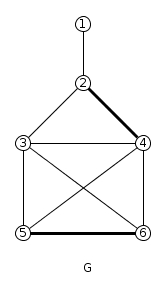
\includegraphics[width=3cm]{grafos_yed/g_47.jpg}
  \caption{$M = \{\{2,4\},\{5,6\}\}$ � um emparelhamento no grafo G.}
  \label{fig:g_47}
\end{figure}

Os v�rtices $2,4,5,6$ s�o ditos cobertos no exemplo da Figura \ref{fig:g_47}.

Um emparelhamento � \textbf{perfeito} se $V(G[M]) = V(G)$, ou seja, se todos os v�rtices do grafo original s�o cobertos por $M$.

Um emparelhamento � \textbf{m�ximo} se n�o exsite emparelhamento maior.

Sua nota��o formal � dada por:

$$ \mu(G) = max\{|M| \therefore M \mbox{ � um emparelhamento em } G\}$$

Temos que o $\mu$ m�ximo para um caminho $P^n$ tal que $n$ � o tamanho do caminho, � $\displaystyle\frac{n}{2}$. Em circuitos emos que o $\mu$ m�ximo $C^n$ tal que $n$ � o tamanho do circuito, � tamb�m $\displaystyle\frac{n}{2}$.

\paragraph*{Observa��o:} Se o n�mero de v�rtices de $G$ for �mpar, um emparelhamento nunca ser� perfeito. Mas o n�mero de v�rtices par n�o garante que exista um emparelhamento perfeito.

Como pode ser observado no grafo $G$ da Figura \ref{fig:g_48}

\begin{figure}[!htb]
  \centering
  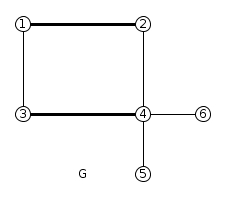
\includegraphics[width=4cm]{grafos_yed/g_48.jpg}
  \caption{N�mero de v�rtices par, que n�o aceitam emparelhamento perfeito.}
  \label{fig:g_48}
\end{figure}

Isso acontece pois os v�rtices $2,4,5,6$ competem por uma mesma aresta. E se um est� o outro n�o pode estar.

\section{Caminho M-Alternante}

$C$ � um caminho \textit{M-Alternante} se � um caminho e suas arestas est�o alternadamente em $M$ e fora de $M$.

\begin{eqnarray*}
  C &=& (v_0, v_1, \ldots, V_k) \mbox{ ent�o } \\
  &\mbox{ ou }& \{V_0,V_1\},\{V_2,V_3\}, \ldots, \{V_{2_i},V_{2_i + 1}\} \\
  &\mbox{ ou }& \{V_1,V_2\},\{V_3,V_4\}, \ldots, \{V_{2_i + 1},V_{2_i + 2}\}
\end{eqnarray*}

s�o arestas em $M$.

\section{Caminho M-Aumentante}

Um caminho \textit{M-Alternante} $C = (V_0, V_1, V_2, \ldots, V_k)$ tal que $K$ seja impar e $V_0$ n�o seja coberto por $M$ � um caminho \textit{M-Aumentante}

\section{Teorema do Caminho M-Aumentante}

Dado um grafo $G$ e um emparelhamento $M$ em $G$, se existe um caminho \textit{M-Aumentante} $C$ em $G$ ent�o existe um emparelhamento $M'$ em $G$ tal que o tamanho de $M'$ � o mesmo de $M$ mais um. Ou formalmente $|M'| = |M| + 1$.

\paragraph*{Prova do Teorema do Caminho M-Aumentante} Para uma aresta $e \in M$ tal que $e$ n�o usa v�rtices de $C$ coloque $e$ e, $M'$. As arestas de $C$ que n�o s�o de $M$ entram em $M'$.

Ou seja, se existe um emparelhamento M-Aumentante, ent�o existe um outro emparelhamento equivalente a esse, entretanto possui uma aresta a mais.

\paragraph*{Observa��es:} N�o existe uma aresta $e$ que pertence a $M$ e que usa v�rtices de $C$ que n�o estejam em $C$.

As arestas de $C$ que n�o est�o em $M$ n�o compartilham v�rtices com as arestas de $M$ que n�o usam v�rtices de $C$.

Para provar a volta do teorema, ou seja, provar que: sendo $G$ um grafo e $M$ um emparelhamento em $G$, $M$ � m�ximo se e somente se n�o existe um caminho \textit{M-Aumentante} em $G$.

Para isso, definimos como $M*$  um emparelhamento m�ximo em $G$.

Seja $H = G[M \cup M*]$, ent�o podemos afirmar que o n�mero m�ximo de arestas para o subgrafo $H$ � dado por $\Delta(H) \leqslant 2$, pois $H$ pode conter ou arestas vindas de $M$, ou arestas vindas de $M*$, as arestas que coincidem s�o desconsideradas.

Com isso pode-se perceber que $H$ cont�m apenas:

\begin{itemize}
    \item v�rtices isolados e desconexos;
    \item arestas isoladas e desconexas;
    \item caminhos e ciclos:
    \begin{itemize}
	\item de tamanho �mpar;
	\item de tamanho par;
    \end{itemize}
\end{itemize}

Como a inten��o � provar que o $|M^*| > |M|$ ent�o descarta-se: v�rtices isolados e arestas isoladas, pois n�o contribuir�o para a contagem.

S�o componenetes conexas de $H$: caminhos e ciclos.

Nos ciclos pares o n�mero de arestas de $M$ � igual ao n�mero de arestas de $M^*$ ent�o podem ser descartados.

Nos ciclos �mpares uma aresta sempre ficar� de fora, logo tamb�m podem ser descartados.

Os caminhos de tamanho par tem o n�mero de arestas de $M$ e de $M^*$ igual, ent�o tamb�m podem ser descartados.

Os caminhos de tamanho �mpar podem ter:

\begin{enumerate}
 \item \label{are:m*} mais arestas de $M^*$ do que de $M$;
 \item \label{are:m} mais arestas de $M$ do que de $M^*$;
\end{enumerate}

Logo pode-se deduzir que somente a afirma��o \ref{are:m*} � verdadeira, pois inicia-se com arestas que est�o em $M^*$, ent�o $M^*$ � aumentante e $M$ n�o � m�ximo.

\section{Diferen�a Sim�trica}

A prova do teorema do caminho \textit{M-Aumentante} pode ser denotada como uma opera��o chamada de \textbf{diferen�a sim�trica}.

Sua nota��o formal � dada por:

$$ M \Delta E(P) = (M \cup E(P)) \smallsetminus (M \cap E(P)) $$

Onde $M$ � o conjunto de arestas do emparelhamento e $E(P)$ � o caminho \textit{M-Aumentante}.

E como o teorema prova, o resultado dessa opera��o � um $M'$ que � um outro emparelhamento em $G$ com uma aresta a mais que $M$.

    %%%%%%%%%%%%%%%%%%%%%%%
% C A P � T U L O   9 %
%%%%%%%%%%%%%%%%%%%%%%%

\chapter{Planaridade}

Um grafo diz-se planar se for poss�vel desenh�-lo de tal forma que duas arestas n�o se cruzem no plano. 

\begin{figure}[!htb]
  \centering
  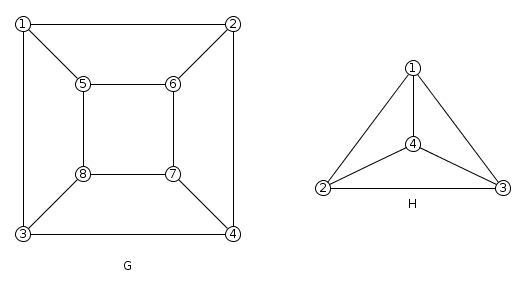
\includegraphics[width=7.5cm]{grafos_yed/g_49.jpg}
  \caption{Grafos Planares}
  \label{fig:g_49}
\end{figure}

O grafo $G$ da Figura \ref{fig:g_49}, temos um cubo planar. O grafo $H$ � um $K^4$ desenhado de forma planar.

\section{Defini��es}

Um grafo planar divide o plano em \textbf{regi�es}, delimitado por suas arestas. Cada uma destas divis�es � denominada por \textbf{face} do grafo.

Dois v�rtices $u$ e $v$ est�o na mesma face, se existe uma aresta $\{u,v\}$ que n�o cruza nenhuma outra aresta do grafo.

No grafo $G$, existem 6 faces, pois a face "exterior" tamb�m � contabilizada. Essa face esta � denominada por face infinita, ou face exterior.

Um grafo $I$ pode ser semelhante $~$ a um grafo $I'$ ou formalmente $I ~ I'$, se a disposi��o de seus v�rtices e arestas n�o alteram suas faces.

Para exemplificar a semelhan�a entre os grafos planares, os grafos $I$ e $I'$ da Figura \ref{fig:g_51} mostram um exemplo.

\begin{figure}[!htb]
  \centering
  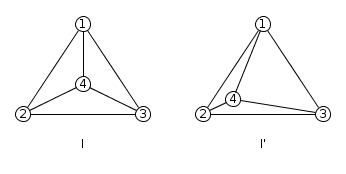
\includegraphics[width=6cm]{grafos_yed/g_51.jpg}
  \caption{Grafos Planares Semelhantes}
  \label{fig:g_51}
\end{figure}

\section{Teorema de Kuratowski}

O teorema diz que $G$ � planar se e somente se n�o existe $H$ que � subgrafo de $G$ que seja uma subdivis�o do grafo completo $K_5$ ou do grafo $K_{3,3}$.

Com isso, sempre que identificarmos subgrafos do tipo $K_5$ ou $K_{3,3}$ podemos descatar a possibilidade da constru��o planar do grafo.

Os grafos $K_5$ ou $K_{3,3}$ est�o dispostos respectivamente como $G$ e $H$ na Figura \ref{fig:g_50}.

\begin{figure}[!htb]
  \centering
  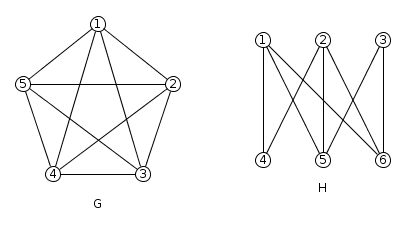
\includegraphics[width=6cm]{grafos_yed/g_50.jpg}
  \caption{Grafos Planares}
  \label{fig:g_50}
\end{figure}

\section{Algoritmo de Hopcroft Tarjan}

Em 1974, Hopcroft e Tarjan apresentaram o primeiro algoritmo linear para decidir se um dado grafo � planar. Uma das etapas para a execuss�o do algoritmo � a identifica��o de componentes biconexas de um grafo.

\section{Encontrar Blocos Bi-conexos de um Grafo}

Define-se como um bloco uma componente bi-conexa ou um caso especial definido por uma aresta e dois v�rtices.

Para encontrar esses blocos devemos encontrar as articula��es de um grafo.

Cada um desses blocos formam uma �rvore, e assim podem ser subdivididos.

\subsection{Encontrar as Articula��es}

Para encontrar as articula��es em um grafo devemos definir duas fun��es chamadas de $f$ e $n$ tal que:

$$f: V(G) \rightarrow V(G)$$

$$n: V(G) \rightarrow \mathbb{N}$$

A fun��o $f$ retorna o v�rtice mais pr�ximo da raiz que pode ser alcan�ado a partir de $v$ com $0$ ou mais arestas de �rvore (para baixo) e com apenas $1$ aresta de retorno para cima.

A fun��o $n$ � a dist�ncia da raiz at� o v�rtice em quest�o, utilizando somente arestas de �rvore.

Para exemplificar a utiliza��o das fun��es $f$ e $n$ vamos utilizar o grafo da Figura \ref{fig:g_52}

\begin{figure}[!htb]
  \centering
  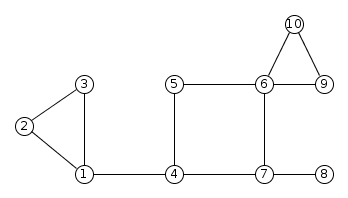
\includegraphics[width=6cm]{grafos_yed/g_52.jpg}
  \caption{Busca por Articula��es}
  \label{fig:g_52}
\end{figure}

A partir desse grafo, podemos gerar o mesmo grafo estruturado de forma diferente com base em uma busca em profundidade. A Figura \ref{fig:g_53} mostra esse novo grafo.

\begin{figure}[!htb]
  \centering
  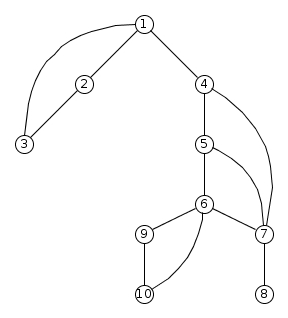
\includegraphics[width=5cm]{grafos_yed/g_53.jpg}
  \caption{Representa��o Estruturada em uma �rvore}
  \label{fig:g_53}
\end{figure}

\paragraph*{Observa��es:} Se um v�rtice $x$ e tem mais que um filho ent�o $x$ � uma articula��o.

Se $x$ n�o � raiz e existe pelo menos um ramo de descendentes sem arestas de retorno para ancestrais de $x$ ent�o $x$ � uma articula��o.

A Tabela \ref{tab:t_2} mostra as fun��es $f$ e $n$ preenchidas para o exemplo da Figura \ref{fig:g_53}.

\begin{table}[!htb]
    \small{
    \centering
      \begin{tabular}{|c|c|c|}
      \hline
      $v$ & $f(v)$ & $n(v)$ \\ 
      \hline
      1 & 1 & 0 \\ 
      \hline
      2 & 1 & 1 \\ 
      \hline
      3 & 1 & 2 \\ 
      \hline
      4 & 4 & 1 \\ 
      \hline
      5 & 4 & 2 \\ 
      \hline
      6 & 4 & 3 \\ 
      \hline
      7 & 4 & 4 \\ 
      \hline
      8 & 8 & 5 \\ 
      \hline
      9 & 6 & 4 \\ 
      \hline
      10 & 6 & 5 \\ 
      \hline
      \end{tabular}
    \caption{Tabela com os valores das fun��es $f$ e $n$ para $v$.}
    \label{tab:t_2}
    }
\end{table}

Para afirmar se um v�rtice $v$ � ou n�o articula��o verifica-se:

Se $n(v) \neq \emptyset$ e existe um filho de $v$ que tem $n(f(w)) \geqslant n(v)$ ent�o $v$ � uma articula��o. Mesmo que essa compara��o funcione apenas para um de seus filhos.

No exemplo os v�rtices $1,4,6,7$ s�o articula��es.

\subsection{Como calcular a Fun��o $f$}

Para calcular a fun��o $f$ temos as seguintes op��es:

\begin{enumerate}
 \item atribuir $v$ - caso inicial;
 \item atribuir $f(w) \therefore w \mbox{ � filho de } v$;
 \item atribuir $u$ se $\{u,w\}$ � uma aresta de retorno partindo de $v$. 
\end{enumerate}

Um poss�vel problema a ser tratado em um algor�tmo recursivo � a quest�o de como saber o $f$ de meu filho se ainda n�o foi calculado. Isso � garantido pela pilha de recurs�o em profundidade.

\section{Aplica��es}

Escrever as aplica��es de planaridade.


	%%%%%%%%%%%%%%%%%%%%%%%%
% C A P � T U L O  1 0 %
%%%%%%%%%%%%%%%%%%%%%%%%

\chapter{Colora��o}

O problema da colora��o em grafos surgiu da necessidade que os desenvolvedores de mapas da antiguidade tinham em obter cores diferentes. Quanto menos cores pudessem usar, melhor. Para colorir os mapas usavam cores de modo que nenhuma regi�o que tivesse fronteira com outra ficasse com a mesma cor. Com isso perceberam que utilizando 4 cores era poss�vel colorir todo o mapa, mas esse questionamento perdurou por muito tempo at� que fosse provado em 2004.

Como os mapas formam grafos planares, tem-se ent�o o teorema das 4 cores.

\section{Teorema das 4 Cores}

Se $G$ � um grafo planar, ent�o pode ser colorido com $4$ cores.

A prova do teorema � complicada e n�o se aplica no alvo de estudos desse livro.

\section{Defini��o de Colora��o}

Dado um grafo $G$, define-se como uma colora��o, uma fun��o $c : v(G)$ tal que se $\{u,v\} \in E(G)$ ent�o $c(u) \neq c(v)$.

O n�mero de cores de uma colora��o $c$ � o tamanho da imagem de $c$ ou seja: $|c| = |c(V(g))|$.

\paragraph*{Observa��o:} Toda colora��o $c$ de tamanho $k$ pode ser representada (trocada) por $c' : V(G) \rightarrow \{1, \ldots, k\}$. Ou seja, a colora��o pode se representada por um n�mero natural.

\subsection{N�mero Crom�tico}

O n�mero crom�tico de um grafo $G$ � definido por $\chi(G)$ que � o menor n�mero de cores de uma colora��o de $G$.

\paragraph*{Observa��es:} Um ciclo de tamanho par pode ser colorido com duas cores.

Um ciclo de tamanho �mpar pode ser colorido com 3 cores.

\subsection{Conjuntos Independentes}

Uma colora��o $C$ divide o grafo $G$ em conjuntos independentes, para cada cor $i$ o conjunto indepentende $C^{-1}(i)$, ou seja, todo $v \in V(G) \therefore C(v) = i$ � um conjunto independente. Ou seja, classificar um grafo em conjuntos independentes � tamb�m colori-lo, pois o n�mero de conjuntos independentes de um grafo � tamb�m seu n�mero crom�tico.

\subsection{Teorema da Colora��o para Grafos Bipartidos}

Todo grafo bipartido se pinta com duas cores.

\paragraph*{Prova:} Como um grafo bipartido separa dois conjuntos de v�rtices que n�o possuem arestas entre s�, pode-se inferir que os elementos do mesmo conjunto podem estar em uma mesma colora��o.

\subsection{Teorema da Colora��o para Grafos K-partidos}

Todo grafo k-partido pode ser pintado com $\chi(G) = k$.

\paragraph*{Prova:} Assim como o grafo bipartido um k-partido possui $k$ conjuntos de v�rtices que n�o possuem arestas entre s�, ou seja, $k$ conjuntos independentes. Com isso infere-se $k$ colora��es.

\subsection{Teorema da Clique M�xima}

O n�mero crom�tico de $G$ � maior ou igual a clique m�xima de $G$. Ou formalmente, $\chi(G) \geqslant \omega(G)$.

\subsection{Teorema  do Conjunto Independente M�ximo}

O n�mero crom�tico de $G$ � menor ou igual a $\displaystyle \frac{n}{\alpha(G)}$. Ou formalmente, $\displaystyle \chi(G) \leqslant \frac{n}{\alpha(G)}$.

\section{Grafos Perfeitos}

Um grafo � dito perfeito se $\chi(G) = \omega(G)$, ou seja quando seu n�mero crom�tico � igual a clique m�xima em $G$. A classifica��o desses grafos � interessante pois, apesar de muitos algoritmo estarem na classe de dificuldade de resolu��o $np$, quando se detecta um grafo perfeito � poss�vel resolver muitos dos algoritmos estudados em tempo polinomial.

\section{Aplica��es}

Escrever as aplica��es de colora��o.
	
	%%%%%%%%%%%%%%%%%%%%%%%%
% C A P � T U L O  1 1 %
%%%%%%%%%%%%%%%%%%%%%%%%

\chapter{Fluxo em Redes}

Os fluxos em redes, s�o estudados normalmente em um tipo de grafo n�o abordado com profundidade nesse livro, os \emph{grafos dirigidos}. Um grafo � dito dirigido se ele possui um par \textbf{ordenado} de v�rtices de tal forma que uma aresta possui um certo sentido. Ent�o podemos dizer que a aresta $\{u,v\}$ se torna diferente (nesse caso) da aresta $\{v,u\}$. Os fluxos tem comportamento ainda melhor com \emph{grafos orientados}. Um grafo � dito orientado se o sentido de suas arestas n�o forma um ciclo no grafo, ou seja, uma aresta que aponta para um sucessor de um v�rtice $v$ n�o ter� nenhum de seus sucessores que apontam para um predecessor de $v$.

Ao se trabalhar com Fluxo em Redes, ainda � necess�rio atribuir pesos nas arestas de tal forma que um grafo $G = (V,E,\omega)$ tal que $\displaystyle E = \binom{V}{2}$ e $E$ � um par ordenado. $\omega : E \rightarrow \mathbb{R}$ � uma fun��o que atribui um peso a cada aresta.

\paragraph*{Nota��o:} Arestas em grafos dirigidos s�o chamadas de arcos.

\section{Defini��es}

Os fluxos est�o intimamente ligados com os pesos nas arestas que incidem em determinado v�rtice. Suponha dado um grafo dirigido $G$ e uma fun��o $\omega$ que atribui um n�mero inteiro a cada arco de $G$. Diremos que o valor de $\omega$ num arco � o \emph{fluxo no arco}. Para qualquer v�rtice $v$ de $G$, o \emph{influxo} (denotado por $inf$) em $v$ � a soma dos fluxos nos arcos que entram em $v$. O \emph{efluxo} (denotado por $ef$) de $v$ � a soma dos fluxos nos arcos que saem de $v$.

O saldo em $v$ � a diferen�a do \emph{efluxo} com o \emph{influxo}.

$$ S = ef(v) - inf(v) $$

Portando, o saldo em $v$ � o que sai de $v$ menos o que entrou em $v$.

\paragraph*{Observa��o:} N�o confundir com a diferen�a $inf(v) - en(v)$.

\section{Fluxo M�ximo}

O problema a ser estudado solicita que se encontre o \emph{fluxo m�ximo}, que pode ser identificado entre dois v�rtices, aqui nomeados de $s$ e $t$.

Encontrar o fluxo m�ximo diz respeito a encontrar o m�ximo de fluxo que $t$ poder� receber a partir de $s$ levando em considera��o os pesos estipulados pela fun��o $\omega$.

\begin{figure}[htbp]
	\centering
		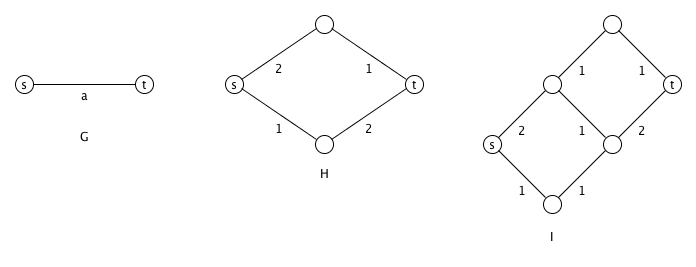
\includegraphics[height=5cm]{grafos_yed/g_54.jpg}
	\caption{caption}
	\label{fig:54}
\end{figure}

A Figura \ref{fig:54} mostra exemplos de fluxos.

No grafo $G$ da Figura \ref{fig:54} fica claro que o fluxo m�ximo de $t$ partindo de $s$ � $a$. No grafo $H$ pode-se observar que o fluxo m�ximo que chega em $s$ � 2. Pois o \textbf{fluxo m�ximo � limitado pelo menor peso do caminho escolhido entre $s$ e $t$}. No grafo $I$ podemos observar que o fluxo que chega em $t$ � no m�ximo 3.

\paragraph*{Observa��o:} Os v�rtices escolhidos para fazer o papel de $s$ e $t$ n�o precisam ter quaisquer propriedades especiais. Na pr�tica, entretanto, n�o h� mal em supor que $s$ � uma fonte e $t$ � um sorvedouro. Poder�amos at� mesmo supor que $s$ � a �nica fonte e $t$ o �nico sorvedouro do grafo dirigido.

\section{Corte M�nimo}

Uma outra defini��o mais restrita para corte se d� por: Dado um grafo dirigido com v�rtice inicial $s$ e v�rtice final $t$, um  corte � qualquer parti��o $E = (A,B)$ do conjunto de v�rtices tal que $s$ est� em $A$ e $t$ est� em $B$.

Em um grafo com peso nas arestas o corte m�nimo � definido por um corte $E(S,\overline{S})$ tal que esse corte seja feito onde minimize-se o custo das arestas.

\subsection{Teorema do Corte}

Qualquer corte $E(s,t)$ � maior ou igual ao fluxo entre $(s,t)$. Isso pois em qualquer corte feito no grafo, o n�mero resultante da somat�ria das arestas do corte nunca poder� ser maior que o fluxo final que $t$ ir� receber.

\subsection{Teorema do Fluxo M�ximo}

O fluxo m�ximo � igual ao corte m�nimo.

\section{Algoritmo de Ford e Fulkerson}

O algoritmo foi publicado por Ford e Fulkerson em 1962, e prop�e que se encontre caminhos de $s$ a $t$ de modo que esses caminhos possam ser modificados de forma a achar o corte m�nimo e consequentemente o fluxo m�ximo.









%%%%%%%%%%%%%%%%%%%%%
% A P � N D I C E S % 
%%%%%%%%%%%%%%%%%%%%%

    \appendix

    %%%%%%%%%%%%%%%%%%%%%%%
% A P � N D I C E - A %
%%%%%%%%%%%%%%%%%%%%%%%

\chapter{Defini��es de S�mbolos}

\begin{itemize}
    \item $\mathbb{N}$ denota o conjunto dos n�meros naturais;
    \item $\mathbb{Z}$ denota o conjunto dos n�meros inteiros;
    \item $\mathbb{Q}$ denota o conjunto dos n�meros racionais;
    \item $\mathbb{R}$ denota o conjunto dos n�meros reais;
    \item $\mathbb{R}^+$ denota o conjunto dos n�meros reais positivos;
    \item $|X|$ denota a cardinalidade do conjunto X;
    \item para $X \subseteq V$ denotamos por $\overline{X}$ o complemento de $X$ em $V$ , isto �, o conjunto $\frac{X}{V}$;
    \item $\binom{V}{2}$ denota o conjunto dos subconjuntos de $V$ de cardinalidade 2: $$ \binom{V}{2} = {X \subseteq V : |X| = 2} $$
    \item $\therefore$ representa \textit{tal que};
\end{itemize}

    %%%%%%%%%%%%%%%%%%%%%%%%
% A P � N D I C E - B %
%%%%%%%%%%%%%%%%%%%%%%%

\chapter{Exerc�cios Resolvidos}

\begin{enumerate}

    \item \label{ex:quimico} Um quimico deseja embarcar os produtos $A,B,C,D,E,F,X$ usando o menor n�mero de caixas poss�vel. Alguns produtos n�o podem ser colocados em uma mesma caixa por que reagem. Os produtos $A,B,C,X$ reagem dois-a-dois e ainda, $A$ reage com $F$ e tamb�m com $D$ (e vice-versa); $E$ reage com $F$ e com $D$ (e vice-versa). Descreva o grafo que modela essa situa��o, mostre um diagrama desse grafo e use esse grafo para descobrir o menor n�mero de caixas necess�rias para embarcar os produtos com seguran�a.

	Para resolver esse exerc�cio, precisamos primeiramente montar um grafo, tendo os produtos como v�rtices e as arestas como rea��es, ou seja um grafo $G$ mostra quais produtos reagem com quais.

	Definindo formalmente $G$, temos:

	\begin{eqnarray*}
	    G    &=& (V,E)\\
	    V(G) &=& \{A,B,C,D,E,F,X\} \\
	    E(G) &=& \{\{A,B\},\{A,C\},\{A,D\},\{A,F\},\{A,X\},\\
		    && \{B,C\},\{B,X\},\{C,X\},\{D,E\},\{E,F\}\}
	\end{eqnarray*}

	Graficamente temos:

	\begin{figure}[!htb]
	    \centering
	    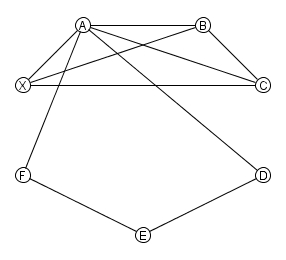
\includegraphics[width=4.5cm]{grafos_yed/g_12.jpg}
	    \caption{Representa��o gr�fica do grafo $G$.}
	    \label{fig:g_12}
	\end{figure}

	De $G$, podemos achar seu complementar $\overline{G}$, que representa quais os produtos \textbf{podem} ir na mesma caixa, ent�o temos:

	\begin{eqnarray*}
	    \overline{G}    &=& (V,E)\\
	    V(\overline{G}) &=& \{A,B,C,D,E,F,X\} \\
	    E(\overline{G}) &=& \{\{A,E\},\{B,D\},\{B,E\},\{B,F\},\{C,D\},\\
			      && \{C,E\},\{C,F\},\{D,F\},\{D,X\},\{E,X\},\\
			      && \{F,X\}\}
	\end{eqnarray*}

	Graficamente temos:

	\begin{figure}[!htb]
	    \centering
	    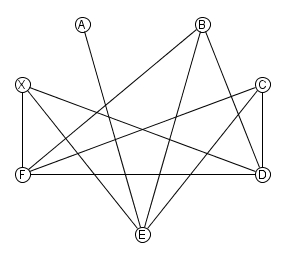
\includegraphics[width=4.5cm]{grafos_yed/g_13.jpg}
	    \caption{Representa��o gr�fica do grafo $\overline{G}$.}
	    \label{fig:g_12}
	\end{figure}

	Com o grafo $\overline{G}$ basta pegar um produto e seguir quais produtos reagem com ele ou n�o. Em um caminho se um produto $Y$ pode ir na mesma caixa que um produto $W$, ent�o devemos verificar se mais algum produto pode ir com $Y$ e $W$.

	Iniciando a navega��o pelo grafo por $A$, podemos observar que ele pode ser colocado com o elemento $E$, mas o elemento $E$, n�o permite que nenhum outro produto seja colocado na mesma caixa. Partindo do produto $B$, podemos coloca-lo na mesma caixa que $D$ e ainda na mesma caixa seria poss�vel colocar $F$ que est� ligada a ambos. $C$ s� pode ir na mesma caixa dos produtos que j� foram colocados, e n�o pode ir com $X$. Ent�o separamos em outras 2 caixas $X$ e $C$.

	Logo, o n�mero m�nimo de caixas � 4, dispostas:

	\begin{enumerate}
	    \item Caixa 1 = $\{A,E\}$
	    \item Caixa 2 = $\{B,D,F\}$
	    \item Caixa 3 = $\{C\}$
	    \item Caixa 4 = $\{X\}$
	\end{enumerate}


    \item Para todo $n \in \mathbb{N}$, qual o m�ximo de arestas que um grafo com $n$ v�rtices pode ter?

	Um grafo � definido por $G=(V,E)$ tal que $E \subseteq \binom{V}{2}$.

	Isso significa o n�mero de vezes que se consegue extrair 2 de $V$, ou a combina��o de 2 em 2 de v�rtices.

	Temos:

	$$ \Big|\binom{V}{2}\Big| = \Big( \binom{|V|}{2}\Big) = $$

	$$ \frac{|N|!}{2!(|N|-2)!} = \frac{|N|(|N|-1)}{2} = \frac{|N|^2-2}{2} $$

    \item D� o complemento dos seguintes grafos:

	\begin{enumerate}
	    \item
	    \begin{eqnarray*}
		V(\overline{G}) &=& \{1,2,3,4,5,6,7\} \\
		E(\overline{G}) &=& \{\{1,2\}, \{1,3\}, \{2,4\}, \{2,5\}, \{3,6\}, \\
				  && \{3,7\}\}
	    \end{eqnarray*}

	    Para achar o grafo complementar basta aplicar a defini��o:
	    \begin{eqnarray*}
		V(\overline{G}) &=& V(G) \\
		E(\overline{G}) &=& \{\{u,v\} \subset V(G): \{u,v\} \not\in\ E(G)\}
	    \end{eqnarray*}
	    assim, obtemos:
	    \begin{eqnarray*}
		V(\overline{G}) &=& \{1,2,3,4,5,6,7\} \\
		E(\overline{G}) &=& \{\{7,1\}, \{7,2\}, \{7,4\}, \{7,5\}, \{7,6\}, \\
				  && \{6,5\}, \{6,4\}, \{6,2\}, \{6,1\}, \{5,4\}, \\
				  && \{5,3\}, \{5,1\}, \{4,3\}, \{4,1\}, \{3,2\}\}
	    \end{eqnarray*}

	    Os grafos est�o representados graficamente na Figura \ref{fig:g_6}. O grafo $a$ � o grafo definido e o grafo $b$ � o seu grafo complementar.

	    \begin{figure}[!htb]
		\centering
		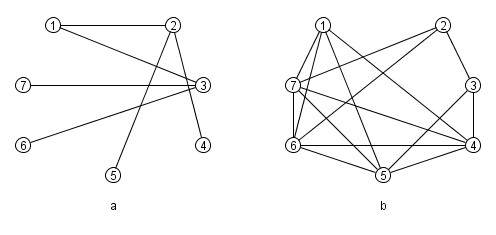
\includegraphics[width=6.5cm]{grafos_yed/g_6.jpg}
		\caption{Grafo complementar}
		\label{fig:g_6}
	    \end{figure}

	    \item
	    \begin{eqnarray*}
		V(\overline{G}) &=& \{1,2,3,4,5\} \\
		E(\overline{G}) &=& \{\{1,2\}, \{1,3\}, \{1,4\}, \{1,5\}, \{2,3\}, \\
				  && \{2,4\}, \{2,5\}, \{3,4\}, \{3,5\}, \{4,5\}\}
	    \end{eqnarray*}
	    Como o grafo acima � um grafo completo, seu grafo complementar ($\overline{G}$) � dado por:
	    \begin{eqnarray*}
		V(\overline{G}) &=& \{1,2,3,4,5\} \\
		E(\overline{G}) &=& \{\}
	    \end{eqnarray*}
	\end{enumerate}


    \item Se temos a uni�o dos grafos $G$ e $H$ por $G \cup H = V(G) \cup V (H), E(G) \cup E(H)$. A uni�o $G \cup H$ � um grafo?

	\begin{eqnarray*}
	    G \cup H &=& \{V(G) \cup V(H), E(G) \cup E(H)\}\\
	    V' &=& V(G) \cup V(H)\\
	    E' &=& E(G) \cup V(H)\\
	    E' &=& \binom{V(G)}{2} \cup \binom{V(H)}{2}\\
	    V(G) \cup V(G) &=& V'\\
	    E' &=& \binom{V'}{2}\\
	    I  &=& \{V', \binom{V'}{2}\}
	\end{eqnarray*}

    \item Prove que $G \cup \overline{G} = K^n$:

	Seja um grafo completo: Um grafo � chamado de completo sobre $V$ se todo par de v�rtices de $V$ � uma aresta do grafo.

	Dado determinado $G$ um grafo n�o completo, e $\overline{G}$ seu grafo complementar, tamb�m n�o completo, logo a uni�o de $G$ e $\overline{G}$ garante que o grafo resultante $G_r = G \cup \overline{G}$ tem todos os v�rtices conectados a todos, formando um grafo completo.

	Prova formal:

	Um grafo,

	\begin{eqnarray*}
	    & G(V,E) \\
	    V & = & V|G| \\
	    E & = & E|G| \therefore E \subseteq \binom{V}{2}
	\end{eqnarray*}

	� composto por $V$ e $E$ que s�o os v�rtices e arestas do grafo respectivamente, suas arestas formam um subconjunto de cardinalidade dois, compreendidas por dois v�rtices.

	Um grafo completo � dado por:

	$$E = \binom{V}{2} \therefore E = K^n$$

	Para cada qualquer par de v�rtices de um grafo completo $G_c$ h� uma aresta $v$ que os liga.

	Um grafo complementar � dado por:

	\begin{eqnarray*}
	    V(\overline{G}) & = & V|G| \\
	    E(\overline{G}) & = & \{\{u,v\} \subset V(G) : \{u,v\} \not\in\ E(G)\}\}
	\end{eqnarray*}

	Um grafo complementar $G_c$ possui uma c�pia dos v�rtices do grafo original ($G$) e um v�rtice � ligado a outro se e somente se no grafo original eles n�o s�o ligados.

	Sejam $G$ e $H$ dois grafos distintos, sua uni�o d� origem a um novo grafo $I$.

	\begin{eqnarray*}
	    I = H \cup G &=& (V(G) \cup V(H), E(G) \cup E(H))
	\end{eqnarray*}

	Ent�o,

	\begin{eqnarray*}
	    G \cup \overline{G} &=& (V(G) \cup V(\overline{G}), E(G) \cup E(\overline{G})) \\
	    V(\overline{G}) &=& V(G) \\
	    V(G) &=& V(\overline{G}) = V(G) \\
	    E(\overline{G}) &=& \binom{V(G)}{2} \smallsetminus E(G) \\
	    E(G) \cup E(\overline{G}) &=& E(G) \cup (\binom{V(G)}{2} \smallsetminus E(G)) \\
	\end{eqnarray*}

	Um grafo completo com $V(G)$ como seu conjunto de v�rtices � dado por: $(V(G), \binom{V(G)}{2})$. Ent�o:

	\begin{eqnarray*}
	    G \cup \overline{G} = (V(G), E(G) \cup (\binom{V(G)}{2} \smallsetminus E(G))
	\end{eqnarray*}

	Para que $G \cup \overline{G}$ seja completo � preciso que:

	\begin{eqnarray*}
	    E(G) \cup (\binom{V(G)}{2} \smallsetminus E(G)) = \binom{V(G)}{2} \\
	    \forall e \in E \binom{V(G)}{2}, e \in E(G) \cup E(\overline{G}) ?
	\end{eqnarray*}

	Logo, para qualquer aresta $e$ pertencente ao grafo completo, ou $e$ estar� no conjunto de arestas de $G$ ou no conjunto de arestas de $\overline{G}$

%        \item Considere o caso geral do exerc�cio \ref{ex:quimico}: Um qu�mico deseja embarcar os produtos $p_1,p_2, \ldots ,p_n$ usando o menor n�mero de caixas. Alguns produtos n�o podem ser colocados num mesmo caixas porque reagem. Seja G o grafo que modela esse problema, onde v�rtices s�o produtos e arestas os pares que reagem, e denote por $X(G)$ o n�mero de m�nimo de caixas de modo que seja poss�vel encaixotar os produtos com seguran�a. Prove que:
%
%            $$ X(G) \leq \frac{1}{2} + \sqrt{2m + \frac{1}{4}}$$

    \item Chico e sua esposa foram a uma festa com tr�s outros casais. No encontro deles houveram v�rios apertos de m�o. Ningu�m apertou a pr�pria m�o ou a m�o do(a) esposo(a), e ningu�m apertou a m�o da mesma pessoa mais de uma vez.

	Ap�s v�rios cumprimentos Chico perguntou para todos, inclusive a sua esposa, quantas m�os cada um apertou e recebeu de cada pessoa uma resposta diferente. Pergunta-se, quantas m�os Chico apertou, e quantas m�os a esposa de chico apertou?

	A primeira informa��o relevante para o problema �: "\emph{Ap�s v�rios cumprimentos Chico perguntou para todos, inclusive a sua esposa, quantas m�os cada um apertou e recebeu de cada pessoa uma resposta diferente.}" Isso significa que, nos � dado o vetor de graus para o grafo a ser constru�do, que vai de 0 a 6.

	Ent�o: $vet = \{0,1,2,3,4,5,6\}$

	Ainda � poss�vel descobrir qual o grau do v�rtice que representa chico, pois temos apenas 3 graus �mpares e segundo o Corol�rio 1 na se��o \ref{corolario:1} devemos ter um n�mero par de graus �mpar, ou seja o grau de Chico � impar.

	O pr�ximo passo � desenhar os v�rtices do grafo que representam as pessoas da festa. Representado graficamente pela Figura \ref{fig:g_16}

	\begin{figure}[!htb]
	    \centering
	    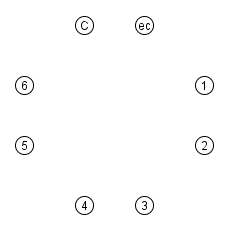
\includegraphics[width=4cm]{grafos_yed/g_16.jpg}
	    \caption{Disposi��o dos casais na festa de Chico.}
	    \label{fig:g_16}
	\end{figure}

	Temos ainda que os c�njuges s�o os pares $\{\{1,2\},\{3,4\},\{4,5\},\{C,ec\}\}$.

	O pr�ximo passo � identificar um padr�o para adicionar as arestas em um v�rtice, pegando aleatoriamente um v�rtice qualquer no grafo, devemos iniciar as liga��es de modo a eliminar todos os graus identificados no vetor de graus.

	O v�rtice $1$ ser� ligado a todos, ent�o ter� o grau $6$. Sendo assim, precisamos identificar algu�m para ser o v�rtice de grau $0$ que s� pode ser a seu c�njuge, pois o v�rtice $1$ j� foi ligado a todos os outros. Eliminamos ent�o os graus $0$ e $6$. Como pode ser visto no grafo da Figura \ref{fig:g_17}

	\begin{figure}[!htb]
	    \centering
	    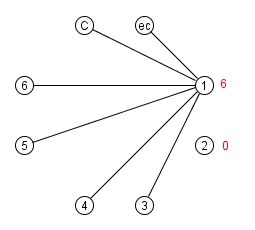
\includegraphics[width=4cm]{grafos_yed/g_17.jpg}
	    \caption{Primeiro casal conectado na festa de Chico.}
	    \label{fig:g_17}
	\end{figure}

	Agora precisamos ligar um outro v�rtice aleat�rio a $5$ pessoas. Note que todos j� tem grau pelo menos 1. Ligamos o v�rtice $4$ a todos os poss�veis, e temos ent�o os v�rtices de graus $5$ e $1$. Pois sua esposa j� tem 1 comprimento e todos os outros agora t�m 2. Como pode ser visto no grafo da Figura \ref{fig:g_18}

	  \begin{figure}[!htb]
	    \centering
	    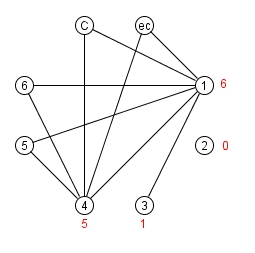
\includegraphics[width=4cm]{grafos_yed/g_18.jpg}
	    \caption{Segundo casal conectado na festa de Chico.}
	    \label{fig:g_18}
	\end{figure}

	O �ltimo casal a ser conectado deve conectar $4$ e $2$ v�rtices. E assim temos o grafo terminado, e podemos identificar o grau de Chico e de sua esposa. Como pode ser visto no grafo da Figura \ref{fig:g_19}

	  \begin{figure}[!htb]
	    \centering
	    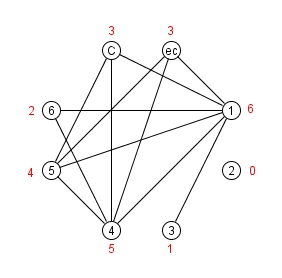
\includegraphics[width=4cm]{grafos_yed/g_19.jpg}
	    \caption{Terceiro casal conectado na festa de Chico.}
	    \label{fig:g_19}
	\end{figure}

	\item Dados os vetores de grau, diga se podemos construir os grafos:

	\begin{enumerate}
	    \item \label{ex:vet_a} $\{2,3,3,4,4,5\}$
	    \item \label{ex:vet_b} $\{2,3,4,4,5\}$
	    \item \label{ex:vet_c} $\{2,2,3,3\}$
	    \item \label{ex:vet_d} $\{1,1,2,2,2\}$
	\end{enumerate}

	O vetor (\ref{ex:vet_a}) n�o pode ser constru�do pois o grau $5$ � igual ou maior que o n�mero de v�rtices do grafo. O vetor (\ref{ex:vet_b}) mostra que a quantidade de graus �mpar � par, ent�o esse grafo tamb�m n�o pode ser constru�do.

	O grafo (\ref{ex:vet_c}) est� disposto na Figura \ref{fig:g_14}:

	\begin{figure}[!htb]
	    \centering
	    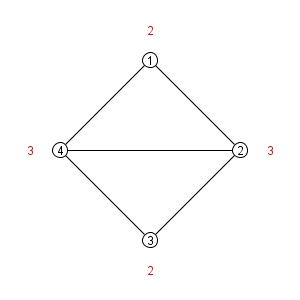
\includegraphics[width=5cm]{grafos_yed/g_14.jpg}
	    \caption{Grafo constru�do a partir do vetor de graus (\ref{ex:vet_c}).}
	    \label{fig:g_14}
	\end{figure}

	O grafo (\ref{ex:vet_d}) pode ser constru�do de 2 formas, representadas pela Figura \ref{fig:g_15}.

	\begin{figure}[!htb]
	    \centering
	    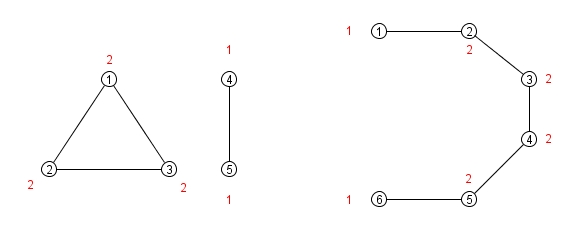
\includegraphics[width=8cm]{grafos_yed/g_15.jpg}
	    \caption{Grafos constru�do a partir do vetor de graus (\ref{ex:vet_d}).}
	    \label{fig:g_15}
	\end{figure}

	Em vermelho, podemos conferir os graus de cada v�rtice.

    \item \label{ex:ind} Seja $G$ um grafo e um conjunto $M \subseteq E(G)$, forme o subconjunto $U = \bigcup_{e \in E}{e}$ de v�rtices de $G$. Prove ou d� um contra-exemplo para $G[U] = G[M]$.

	Seja $G$ um grafo definido por $G = \{1,2,3, \{1,2\},\{2,3\},\{3,1\}\}$.

	Seja $M$ um conjunto de arestas definido por $M = \{\{1,2\},\{2,3\}\}$.

	Se aplicarmos a indu��o $G[M]$ obtemos:

	\begin{eqnarray*}
	    G[M] &=& \{V', M)\}\\
	    V'   &=& \bigcup_{e \in M}e\\
	    V'   &=& \{1,2,3\}\\
	    M    &=& \{\{1,2\},\{2,3\}\}
	\end{eqnarray*}

	Seja um grafo $H$ definido por $H = G[M]$.

	Seja $V$ um conjunto de v�rtices definido por $\{1,2,3\}$.

	Se aplicarmos $G[V]$ obtemos:

	\begin{eqnarray*}
	    G[V] &=& \{V, E'\}\\
	    V    &=& \{1,2,3\}\\
	    E'   &=& \{e \in E(G) \therefore e \subseteq V\}\\
	    E'   &=& \{\{1,2\},\{2,3\},\{3,1\}\}
	\end{eqnarray*}

	Logo:

	\begin{enumerate}
	    \item $G[M]$ � um subgrafo induzido pelas arestas do conjunto $M$.
	    \item $G[V]$ � um subgrafo induzido pelos v�rtices do conjunto $V$.
	    \item $G[V]$ � formado pelas arestas de $M$ e mais a aresta $e = \{3,1\}$, que est� presente em $G$ mas n�o est� presente em $G[M]$.
	\end{enumerate}

	Ent�o, podemos deduzir que $G[V] \neq G[M]$.

	Os grafos est�o representados na Figura \ref{fig:g_23}.

	\begin{figure}[!htb]
	    \centering
	    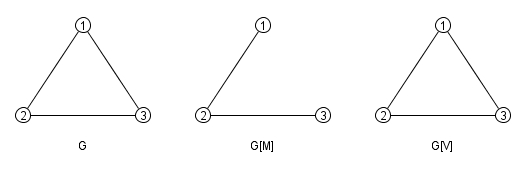
\includegraphics[width=7.5cm]{grafos_yed/g_23.jpg}
	    \caption{Grafos do Exerc�cio \ref{ex:ind}.}
	    \label{fig:g_23}
	\end{figure}


    \item Descubra um grafo induzido de

	\begin{eqnarray*}
	    V(G) &=& \{1,2,3,4,5,6,7,8\}\\
	    E(G) &=& \{\{1,2\},\{1,3\},\{2,3\},\{2,5\},\{3,6\},\\
		      &&\{8,5\},\{8,6\},\{5,6\},\{3,4\},\{5,7\}\}
	\end{eqnarray*}

	1-regular e o maior n�mero poss�vel de arestas.

	Um grafo do tipo 1-regular tem todos seus v�rtices com grau igual a $1$.

	A Figura \ref{fig:g_24} demonstra o grafo $G[1-regular]$.

	\begin{figure}[!htb]
	    \centering
	    \includegraphics[width=7.5cm]{grafos_yed/g_24.jpg}
	    \caption{Grafo $G[1-regular]$.}
	    \label{fig:g_24}
	\end{figure}

    \item Dado os grafos $A$ e $B$ dispostos na Figura \ref{fig:g_25} prove que $A$ � um subgrafo induzido de $B$.

	\begin{figure}[!htb]
	    \centering
	    \includegraphics[width=5cm]{grafos_yed/g_25.jpg}
	    \caption{Grafos $A$ e $B$.}
	    \label{fig:g_25}
	\end{figure}

	\begin{eqnarray*}
	    B &=& (V,E)\\
	    V(B) &=& \{1,2,3,4,5\}\\
	    E(B) &=& \{\{1,2\},\{1,4\},\{1,5\},\{2,3\},\{2,5\}, \\
		      &&\{3,4\},\{3,5\},\{4,5\}\}\\
	    A &=& (V',E')\\
	    V'(A) &=& \{1,2,3,4\}\\
	    E'(A) &=& \{\{1,2\},\{2,3\},\{3,4\},\{1,4\}\\
	    V'(A) &=& S \subseteq V(B)\\
	    E'(A) &=& T \subseteq E(B)\\
	    B[S]  &=& (S,E'')\\
	    B[T]  &=& (V'',T)\\
	    E''   &=& \{e \in E(B) \therefore e \subseteq S\}\\
	    V''   &=& \bigcup_{e \in T}e\\
	    S     &=& \{1,2,3,4\}\\
	    T     &=& \{\{1,2\},\{1,4\},\{4,3\},\{2,3\}\}\\
	\end{eqnarray*}

	Logo, $B[S]$ ou $B[T] = A$.

	\item Prove que $\delta(G) \leqslant d(G) \leqslant \Delta(G)$.

	Seja $G$ um grafo $G(V,E)$, definimos o conjunto $I = \{d_G(u) \therefore u \in V(G)\}$ que � o vetor de graus do grafo definido.

	\begin{eqnarray*}
	    \delta(G) &=& \mbox{min}(I)\\
	    d(G)      &=& \frac{\sum i}{V(G)}\\
	    \Delta(G) &=& \mbox{max}(I)\\
	\end{eqnarray*}

	Logo,

	\begin{itemize}
	    \item[$\delta(G)$]
	    \begin{itemize}
		\item possui o menor elemento de $I$ ou;
		\item � igual a $d(G)$ ou ;
		\item � igual a $\Delta(G)$ ou ;
		\item � igual a ambos;
	    \end{itemize}

	    \item[$d(G)$]
	    \begin{itemize}
		\item � o somat�rio de todos os elementos de $I$ dividido pelo tamanho de $I$;
	    \end{itemize}

	    \item[$\Delta(G)$]
	    \begin{itemize}
		\item possui o maior elemento de $I$ ou;
		\item � igual a $\delta(G)$ ou ;
		\item � igual a $\Delta(G)$ ou ;
		\item � igual a ambos;
	    \end{itemize}
	\end{itemize}

	Nos casos onde todos elementos seriam iguais a $\delta(G)$ ou $\Delta(G)$, ter�amos $d(G) = \delta(G)$ ou $d(G) = \Delta(G)$ respectivamente.

	Ent�o, ou $d(G)$ � igual a $\delta(G)$ ou $\Delta(G)$, ou est� entre eles.

	Logo, $\delta(G) \leqslant d(G) \leqslant \Delta(G)$.

	\item Prove que para $G$ e $H$ sendo isomorfos, temos $\overline{G}$ e $\overline{H}$ tamb�m isomorfos.

	Seja $G$ e $H$ isomorfos, pois:

	\begin{eqnarray*}
	    |V(G)| &=& |V(H)|\\
	    |E(G)| &=& |E(H)|\\
	    d_G(u) \therefore u \in V(G) &=& d_G(v) \therefore v \in V(H)\\
	    \mbox{existe} & & f(G) \rightarrow f(H)
	\end{eqnarray*}

	ou seja, eles t�m o mesmo tamanho do conjunto de v�rtices, o mesmo tamanho do conjunto de arestas, o mesmo vetor de graus e existe uma fun��o bijetora que satisfa�a a condi��o do isomorfismo.

	Se $\overline{G} \cup G = K^n_G$, ent�o $\overline{H} \cup H = K^n_H$ e assim:

	$$ K^n_G \simeq K^n_H$$

	pois:

	\begin{eqnarray*}
	    |V(K^n_G)| &=& |V(K^n_H)|\\
	    |E(K^n_G)| &=& |E(K^n_H)|\\
	    d_G(u) \therefore u \in V(K^n_G) &=& d_G(v) \therefore v \in V(K^n_H)\\
	    \mbox{existe} & & f(K^n_G) \rightarrow f(K^n_H)
	\end{eqnarray*}

	Sejam $A$ e $B$:

	\begin{eqnarray*}
	    A &=& K^n_G \smallsetminus G = \overline{G}\\
	    B &=& K^n_H \smallsetminus G = \overline{H}\\
	\end{eqnarray*}

	Logo, $A \simeq B$ e portanto, $\overline{G} \simeq \overline{H}$.


	\item Seja $G$ um grafo com 14 v�rtices e 25 arestas. Se todo v�rtice de $G$ tem grau 3 ou 5, quantos v�rtices de grau 3 o grafo $G$ possui?

	Partindo do \ref{teo:1} dado por $$ \sum\limits_{u \in V} d_g(u) = 2|E(G)| $$

	Logo poder�amos obter as combina��es:

	\begin{itemize}
	    \item 10 v�rtices com grau 3 e 4 v�rtices com grau 5;
	    \item 15 v�rtices com grau 3 e 1 v�rtices com grau 5;
	    \item 5 v�rtices com grau 3 e 7 v�rtices com grau 5;
	\end{itemize}

	Entretanto somente a combina��o 10 v�rtices com grau 3 e 4 v�rtices com grau 5 resulta em 14 v�rtices.

	O grafo $G$ � demonstrado na Figura \ref{fig:g_30}:

	\begin{figure}[!htb]
	    \centering
	    \includegraphics[width=7cm]{grafos_yed/g_30.jpg}
	    \caption{Grafo $G$}
	    \label{fig:g_30}
	\end{figure}

	\newpage

	\item D� exemplo de um grafo 3-regular que n�o � completo.

	O grafo $G$ � demonstrado na Figura \ref{fig:g_31}:

	\begin{figure}[!htb]
	    \centering
	    \includegraphics[width=3.5cm]{grafos_yed/g_31.jpg}
	    \caption{Grafo $G$}
	    \label{fig:g_31}
	\end{figure}

	\item Prove que em todo grafo de ordem pelo menos 2 existem pelo menos dois v�rtices com o mesmo grau.

	Seja $G$ um grafo, com seu vetor de graus com todos elementos distintos e crescentes, poder�amos ter nesse grafo apenas $n - 1$ graus distintos, ou seja $vet_G = \{0, 1, 2, \ldots, n - 1\}$. Pois se o menor elementos � $0$ ou seja n�o tem nenhuma aresta ligada a ele, ent�o o maior elemento (suposto $n$) n�o poderia ter uma aresta ligada ao v�rtice que tem grau $0$. Com isso esse grafo pode ter no m�ximo grau $n-1$.

	Logo, podemos classificar o $vet_G$ em categorias, que separam graus distintos, o m�ximo de categorias que poderiam ser criadas � $n - 1$ categorias.

	Ent�o, se o tamanho do vetor de graus � $n$ ou seja $|vet_G| = n$ (que tamb�m � o n�mero de v�rtices do grafo) e o m�ximo de categorias com graus distintos que podem se criadas � $n - 1$. Com isso pelo menos 1 grau ir� se repetir.

	Prova por absurdo e exemplo:

	Seja $G = \{1,2,3,4, \{1,2\},\{2,3\}\}$

	Seu vetor de graus � dado por $vet_G = \{0, 1, 1, 2\}$.

	Seja $vet_G = |V(G)| = n = 4$.

	Podemos classificar o grafo dado em 3 categorias de graus distintos, ou seja: $\{0, 1, 2\}$, ent�o $vet_G = n - 1 = 3$.

	Ent�o pelo menos 2 categorias do vetor ir�o se repetir, no exemplo \{1,1\} indicando pelo menos 2 v�rtices com o mesmo grau.

	\item Dado $G$, o grafo linha de $G$, denotado por $LG$, � o grafo cujos v�rtices s�o as arestas de $G$ e um par de v�rtices define uma aresta em $LG$ se, e somente se, esses v�rtices s�o arestas adjacentes em $G$. Dado $G$ determine $|V (LG)|$ e $|E(LG)|$.

	\item Prove que $E(A,B)$ = $E(B,A)$

	\item Mostre que em qualquer grafo $G$ com pelo menos 6 v�rtices ou existe um 3-clique ou existe um 3-conjunto-independente.

\end{enumerate}

\end{document} 